\documentclass[12pt]{article}
\usepackage[english]{babel}
    
%AMS-TeX packages
\usepackage{amssymb,amsmath,amsthm} 
\usepackage{geometry, graphicx}
\usepackage{siunitx}
\usepackage{subcaption}
    
\sisetup{locale=US,group-separator = {,}}
    
\usepackage{pgfplotstable}
\pgfplotsset{compat=1.9}% supress warning
    
% setup the margins
\geometry{margin=1.0in, headheight=15pt}
    
    
\graphicspath{ {../lab02/images} }    
    
\begin{document}
    
\title{PHSX 444: Lab 02; Fourier Transforms}
\author{William Jardee}
\maketitle
    
%% Introduction section. Here I introduce the physics of the experiment and give some slight motivation for the experiment. I personally think that putting the physics of the apparatus here is better. 
\section{Introduction}

    
One of the neatest characteristics of orthogonal basises is how they can be used to recreate a wide range of functions. Probably the most notable of all these basises is the fourier transform. As can be shown through a relatively simple, but clever, derivation, all functions can be written as:
\begin{equation*}
    Y(t) = \int^\infty_{-\infty} y(\omega) \frac{e^{-i\omega t}}{\sqrt{2\pi}} d\omega
    \label{eq:fourier_time}
\end{equation*}
\begin{equation*}
    y(\omega) = \int^\infty_{-\infty} Y(t) \frac{e^{-i\omega t}}{\sqrt{2\pi}} dt
    \label{eq:fourier_freq}
\end{equation*}
This isn't all too useful in application, however. There are two main issues here. The first requiring an exact knowledge of the function to begin with, either in the frequency or time domain. The second being the computation time of finding such a solution to the equation (or the discrete version that we will see soon).
    
To solve the first issue, the Fourier Transform can be rewritten as the Discrete Fourier Transform:
\begin{equation*}
    Y(t) = \sum^{N-1}_{k=0} \Delta t \cdot \frac{e^{i \omega_n t_k}}{\sqrt{2\pi}} y_k 
\end{equation*}
\begin{equation*}
    y(\omega) = \sum^{N-1}_{n=0} \frac{2 \pi}{N \Delta t} \cdot \frac{e^{i \omega_n t_k}}{\sqrt{2\pi}} Y_n
\end{equation*}
Where $\Delta t$ is the time step collected by the data. Now it is possible to translate the time domain of a function to the frequency domain with discrete description of the data. Doing this calculation, especially on the fly, is computationally intensive, requiring $\Omega(N^2)$ time. To beat this, the Fast Fourier Transform (FFT) can be used, achieving O$(N \, \text{ln}N)$ time. A great explanation has been give by Reducible on youtube, which goes into depth on the various steps in implementing the FFT~\cite{youtube}. In order to use this method, there is one stipulation that must be followed: the time must be gathered as a multiple of 2 (i.e. 2, 4, 8, 16, ...). 
    
While the theory behind FFTs is awe-inspiring, it is not at all required for the physicists to implement it. Numpy, the ever-present Python module, offers a weldable version of the algorithm for the layman.
    
It should be noted that when data is being collected to analyze the frequency domain of a function, there are a couple practical limits that must be worried about. If the measured time step is $\Delta t$, and the total duration of measurements is $t_{\text{max}}$, then the frequency step that can be analyzed, $\Delta f = \frac{1}{t_{\text{max}}}$ and the max frequency that information can be resolved for is $f_{\text{max}} = \frac{1}{2 \Delta t}$. This max frequency is also called the Niquest Frequency. Here the trade offs of quick measurements and quality of data have to be analyzed. This is a common trade off that shouldn't at all be surprising to see.
    
%% Experimental Methods section. Here I go into depth about the methods used to collect the data. I also talk about where the apparatus came from. I bring up the way that we will be calibrating the data and collecting enough data to do any trend correction later 
\section{Experimental Methods}
    
The purpose of this lab was to get hands on experience with Fourier Analysis. The first part of the lab was just to collect data outputted from a function generator and in real time analyze it with a spectrum analyzer. The same output was then also collected by an oscilloscope to be analyzed with an FFT method outside of the lab time. In theory, the data collect by both methods should be equivalent. The output of the function generator can also be compared for different settings, seeing how a live analysis compares to one after the fact. One such setting is the window function. If a function being analyzed doesn't look periodic over the realm being measured, it can be manipulate to look pseudo-periodic. One such method is to use the Hanning Window, which is multiplying by a $\text{sin}^2(t)$ that has a period equal to the measurement window. 
    
To test the ability to find a buried frequency in noise, a module fittingly called ``Buried Treasure" was provided. There were four different settings that offered a weak sine wave buried in noise, each progressively getting more difficult. This offered a challenge to underline how to run the interface of the equipment effectively and show the importance of averaging data; a lesson that has been learned.
    
To test practical understanding of the Fourier Methods, an LRC circuit was analyzed. Measurement of the response function were carried out with four different methods, and should all give the same response. We can state this because all four are measuring the same physical system and the only deviation should be because of faulty data collection or mathematical methods. For a general LRC circuit, such as the one in Figure~\ref{fig:circuit}, the expected response is \cite{hyper}:
% http://hyperphysics.phy-astr.gsu.edu/hbase/electric/rlcser.html
\begin{equation*}
    X_C = \frac{1}{\omega C}\quad \text{,} \quad X_L = \omega L \quad \text{,} \quad \omega = \frac{1}{\sqrt{LC}}
\end{equation*}
\begin{equation*}
    Z = \sqrt{R^2 + (X_L - X_C)^2}
\end{equation*}
\begin{equation}
    \text{Phase} = \phi = \text{tan}^{-1}\Big[\frac{X_L-X_C}{R}\Big]
    \label{eq:LRC}
\end{equation}
Where $R$ is the resistor's resistance, $C$ is the capacitor's capacitance, and $L$ is the indicator's inductance. $Z$ is the effect impedance of the three elements together, and $\phi$ is the phase shift that oscillatory inputs experience from the system. 
    
The four methods that will be used to measure will be: 
\begin{enumerate}
    \item Using a single-frequency drive as an input and an oscilloscope and lock-in amplifier to measure the output at several frequencies
    \item Using a noise drive as the input and the spectrum analyzer to measure the output.
    \item Using an Arduino-based network analyzer to sweep over a wide range of frequencies with fine steps to get the amplitude and phase response.
    \item Measuring the transient response using a square wave and applying a FFT to get the transfer function.
\end{enumerate}
    
For the first method, a constant Sine wave was put into the LRC circuit, ranging from 4.1kHz to 5.5kHz with a step size of 0.2kHz. The Sine wave was provided by the function generator and the Sine and Cosine amplitudes were measured using the Lock-In Amplifier. The amplitude of the total response was also measured by an oscilloscope at the same time to ensure the data read by the lock-in amplifier was reliable (all the data can be see in Table~\ref{tab:lock_in_LRC} in Appendix A). 
    
For the second method, a noise drive was taken from the Teach Spin Fourier Methods Electronic Modules system provided in lab. The FFT was then observed in the spectrum analyzer. 
    
For the third method, a wide range of frequencies were provided by an Arduino system, and the response was measured by the same Arduino. This system was provided as a ``black box" that we trust worked, as the data we observed seemed to be reasonable. The Arduino sampled the phase response, both in the Sine and Cosine orientation, and the phase shift. For our trials, the system swept from 1kHz to 10kHz with 100 steps. 
    
The fourth and final method fed the LRC circuit a square wave from the function generator and measured the amplitude and phase of the response by first snapshot-ing the the output with an oscilloscope and applying an FFT to the data post-lab. The square wave, when focused on one half of a period, looks like a step function, thus giving a good understanding of the transient response. 
    
\begin{figure}[!ht]
\centering
	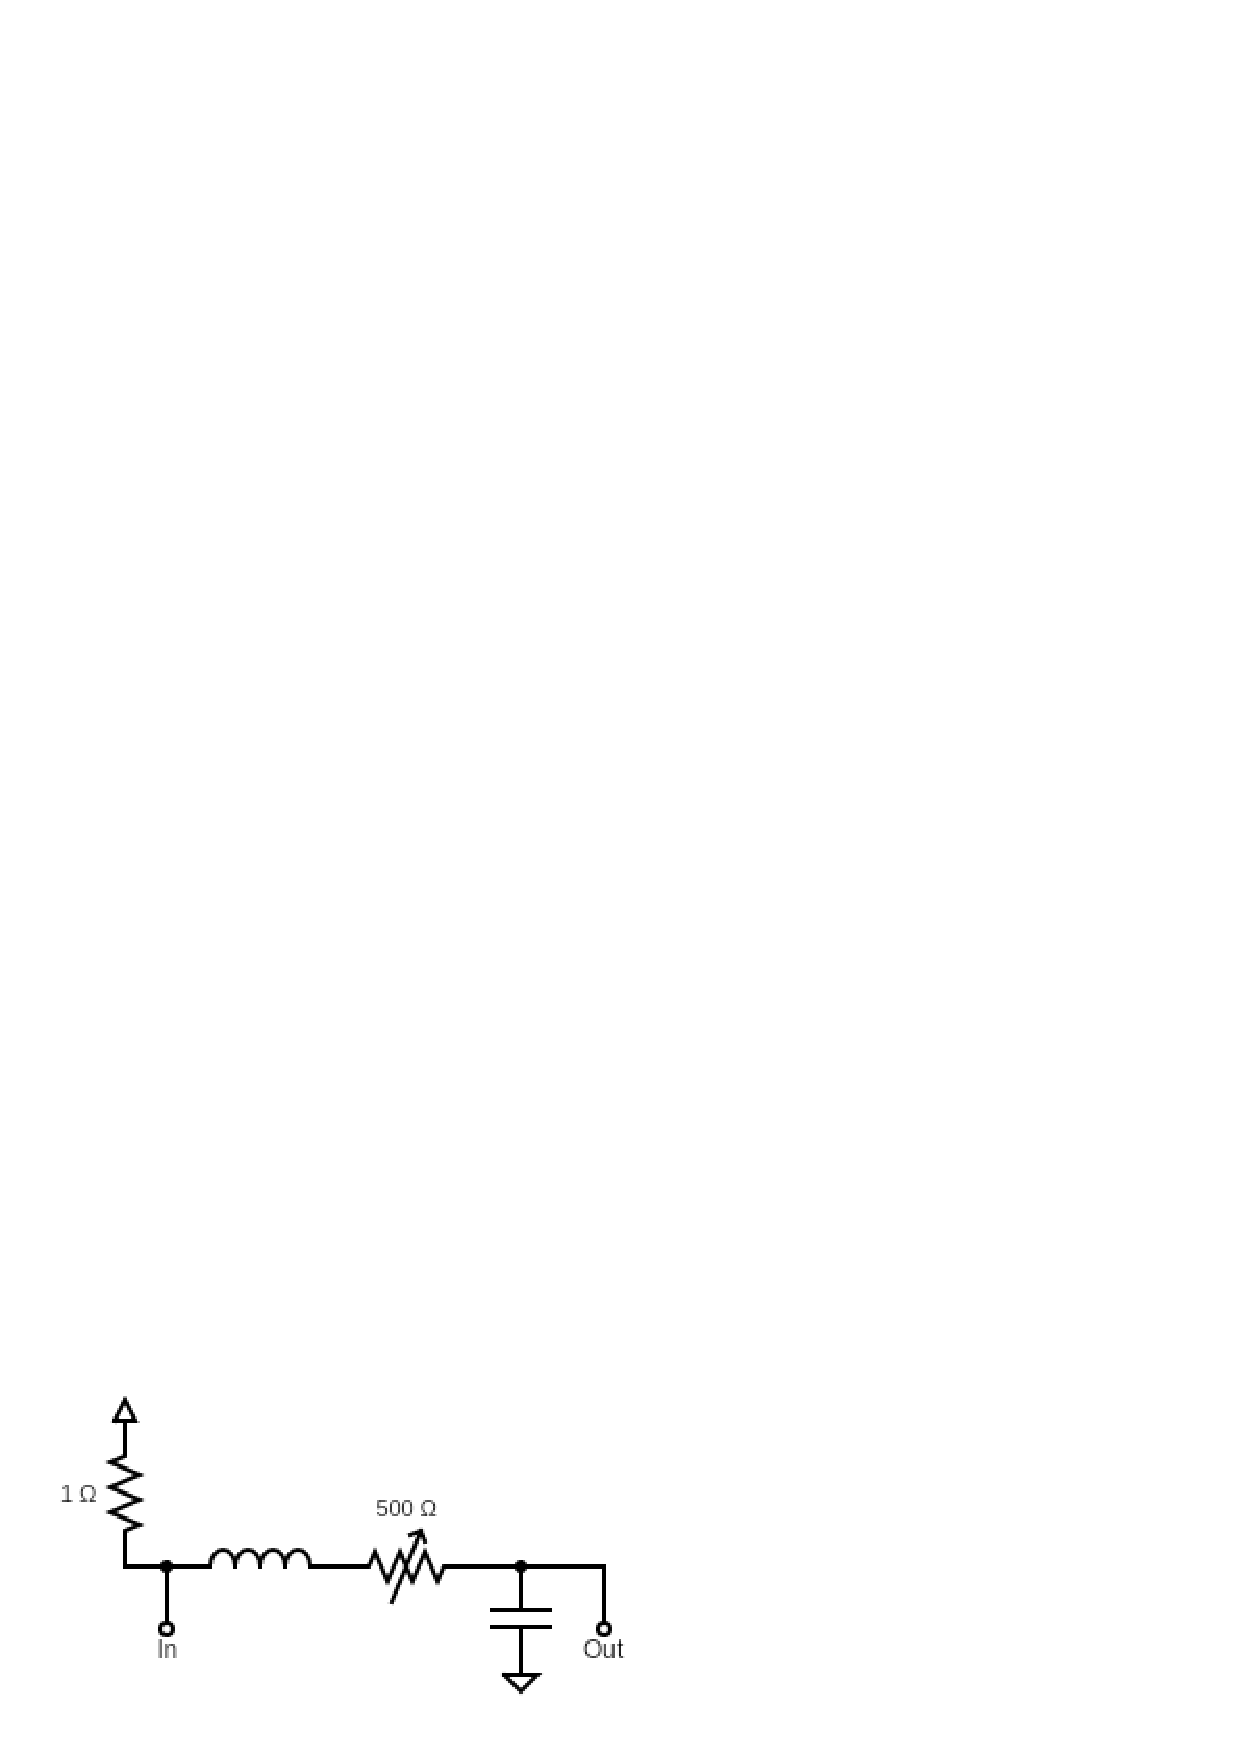
\includegraphics[width=4in]{circuit}
	\caption{The LRC circuit used in the second part of this lab. Diagram created via \cite{circuit}}
	\label{fig:circuit}
\end{figure}
   
The same four methods applied to measure the response function of the LRC circuit were also applied to an acoustical cavity. The acoustical cavity was set up so that a speaker pushed the sound into the bottom of the cylindrical container, and a microphone picked up the volume of the output on the top of the container. The microphone was plugged into the Teach Spin Fourier Methods Electronic Modules system and then fed into the appropriate analysis device; oscilloscope, lock-in amplifier, spectrum analyzer, or arduino system. The acoustical cavity had four possible heights: 3cm, 4cm, 5cm, and 6cm. Each of the four were analyzed. 
    
Tubes have resonance frequencies where the nodes of the sound waves fit well in the tube. If the tubes don't have a wavelength that allows a node to find purchase on the opposite wall, some of the returning waves will destructively interfere with those coming from the speaker. However, when a resonance frequency is achieved, a sharp jump in the surviving amplitude can be observed. Similarly, when nearly all the reflected waves destructively interfere, the amplitude should drop to nearly zero. 
    
For the first measurement method, measurements were taken from 1.3kHz to 4.3kHz with a step size of 0.3kHz. The noise drive was again used for the second method. The third method swept over a frequency of 0kHz (this was an option available for the Arduino, however it is hard to decipher what this data point actually means) to 10kHz with a step size of 500Hz and a drive amplitude of 0.95V. There were two sweeps taken to average the results. The same method to measure the transient response was used. 
    
To save some time, only the 6cm cavity was used to measure the first method. The second and fourth methods used all four cavity sizes. Data was taken for the third method in all four cavity sizes; however, the data for the 3cm cavity was somehow lost in the process and will thus be excluded from the analysis.
    
\begin{figure}[!ht]
    \centering
    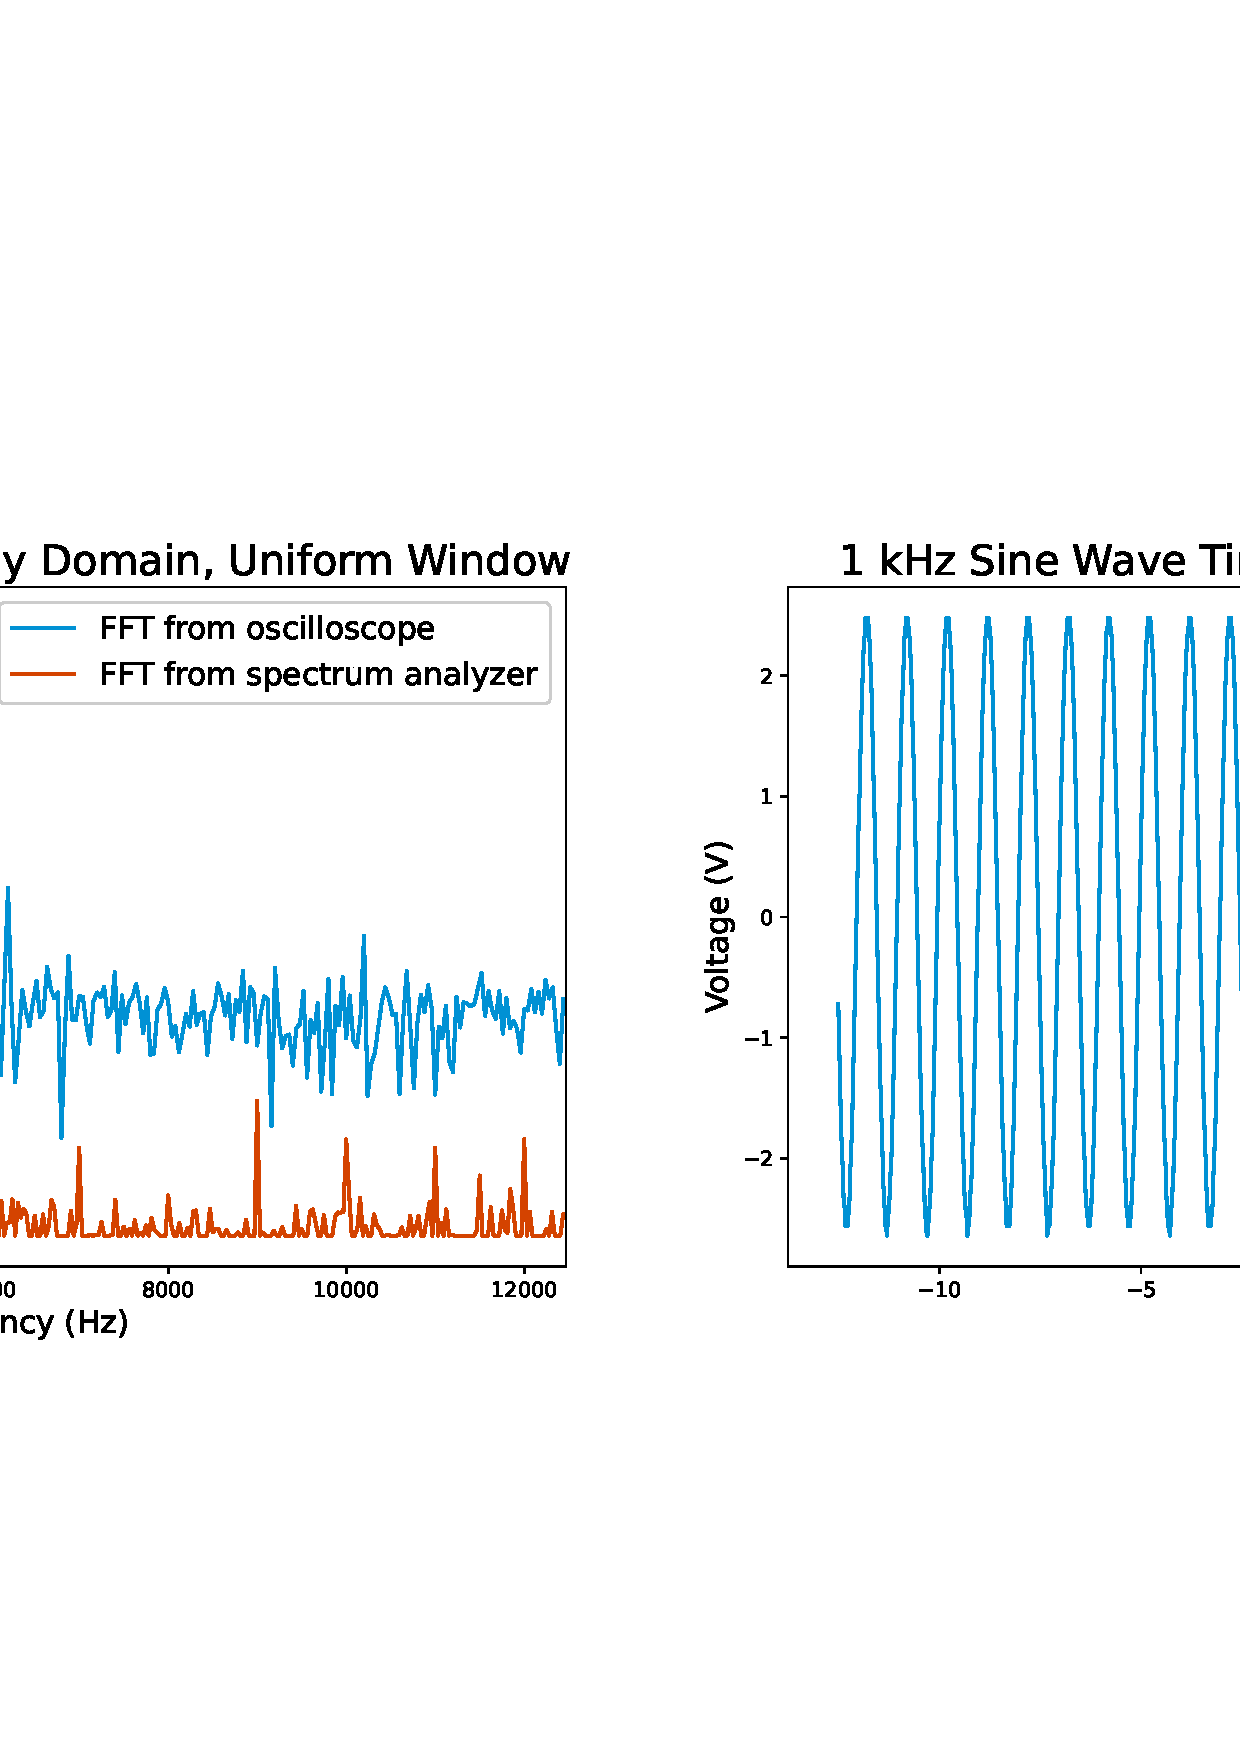
\includegraphics[width=\textwidth]{1 kHz Sine Wave (uniform)}
    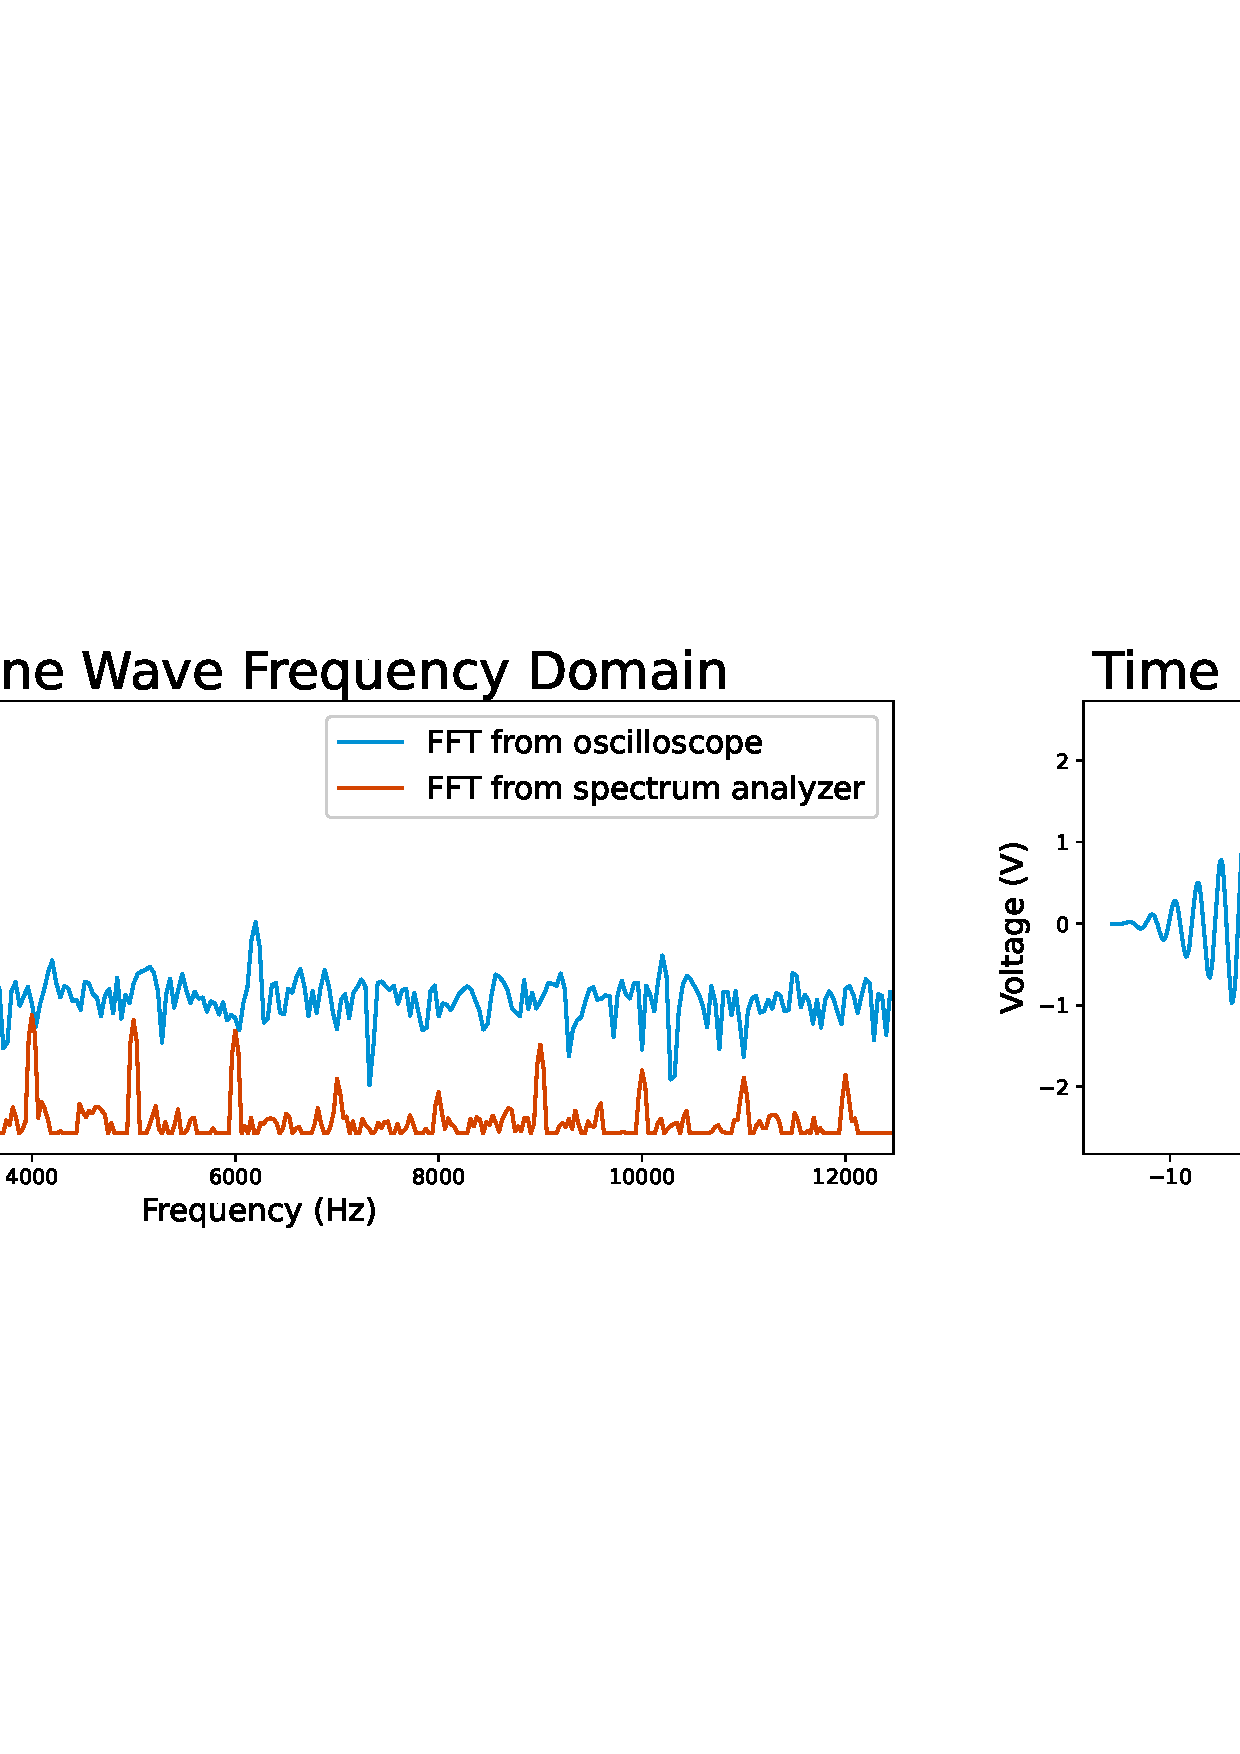
\includegraphics[width=\textwidth]{1 kHz Sine Wave (hanning)}
    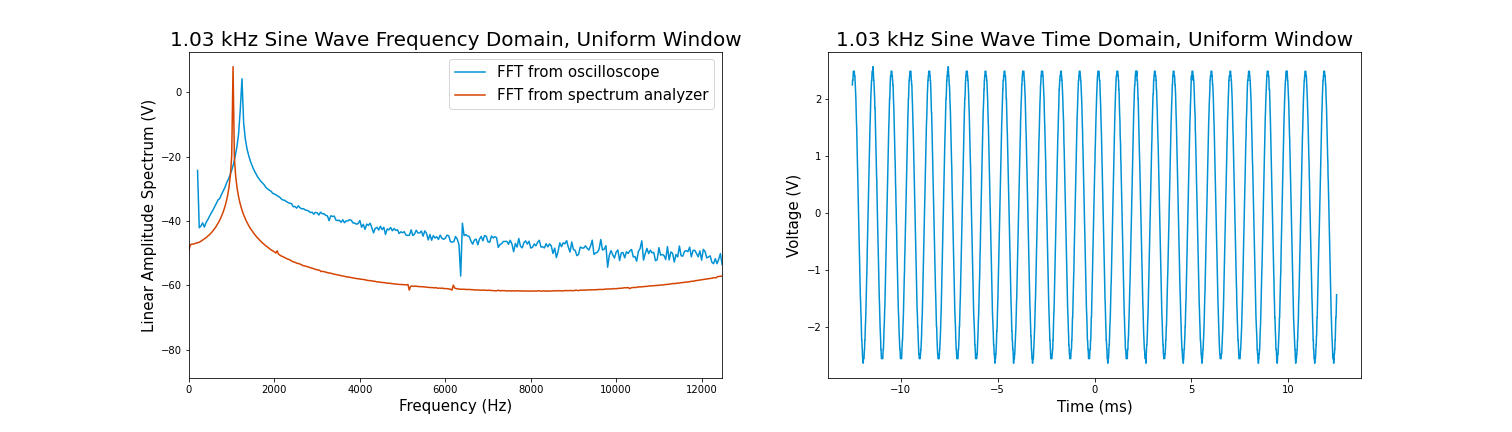
\includegraphics[width=\textwidth]{1_03 kHz Sine Wave (uniform)}
    \label{fig:1.03_sine_uniform}
    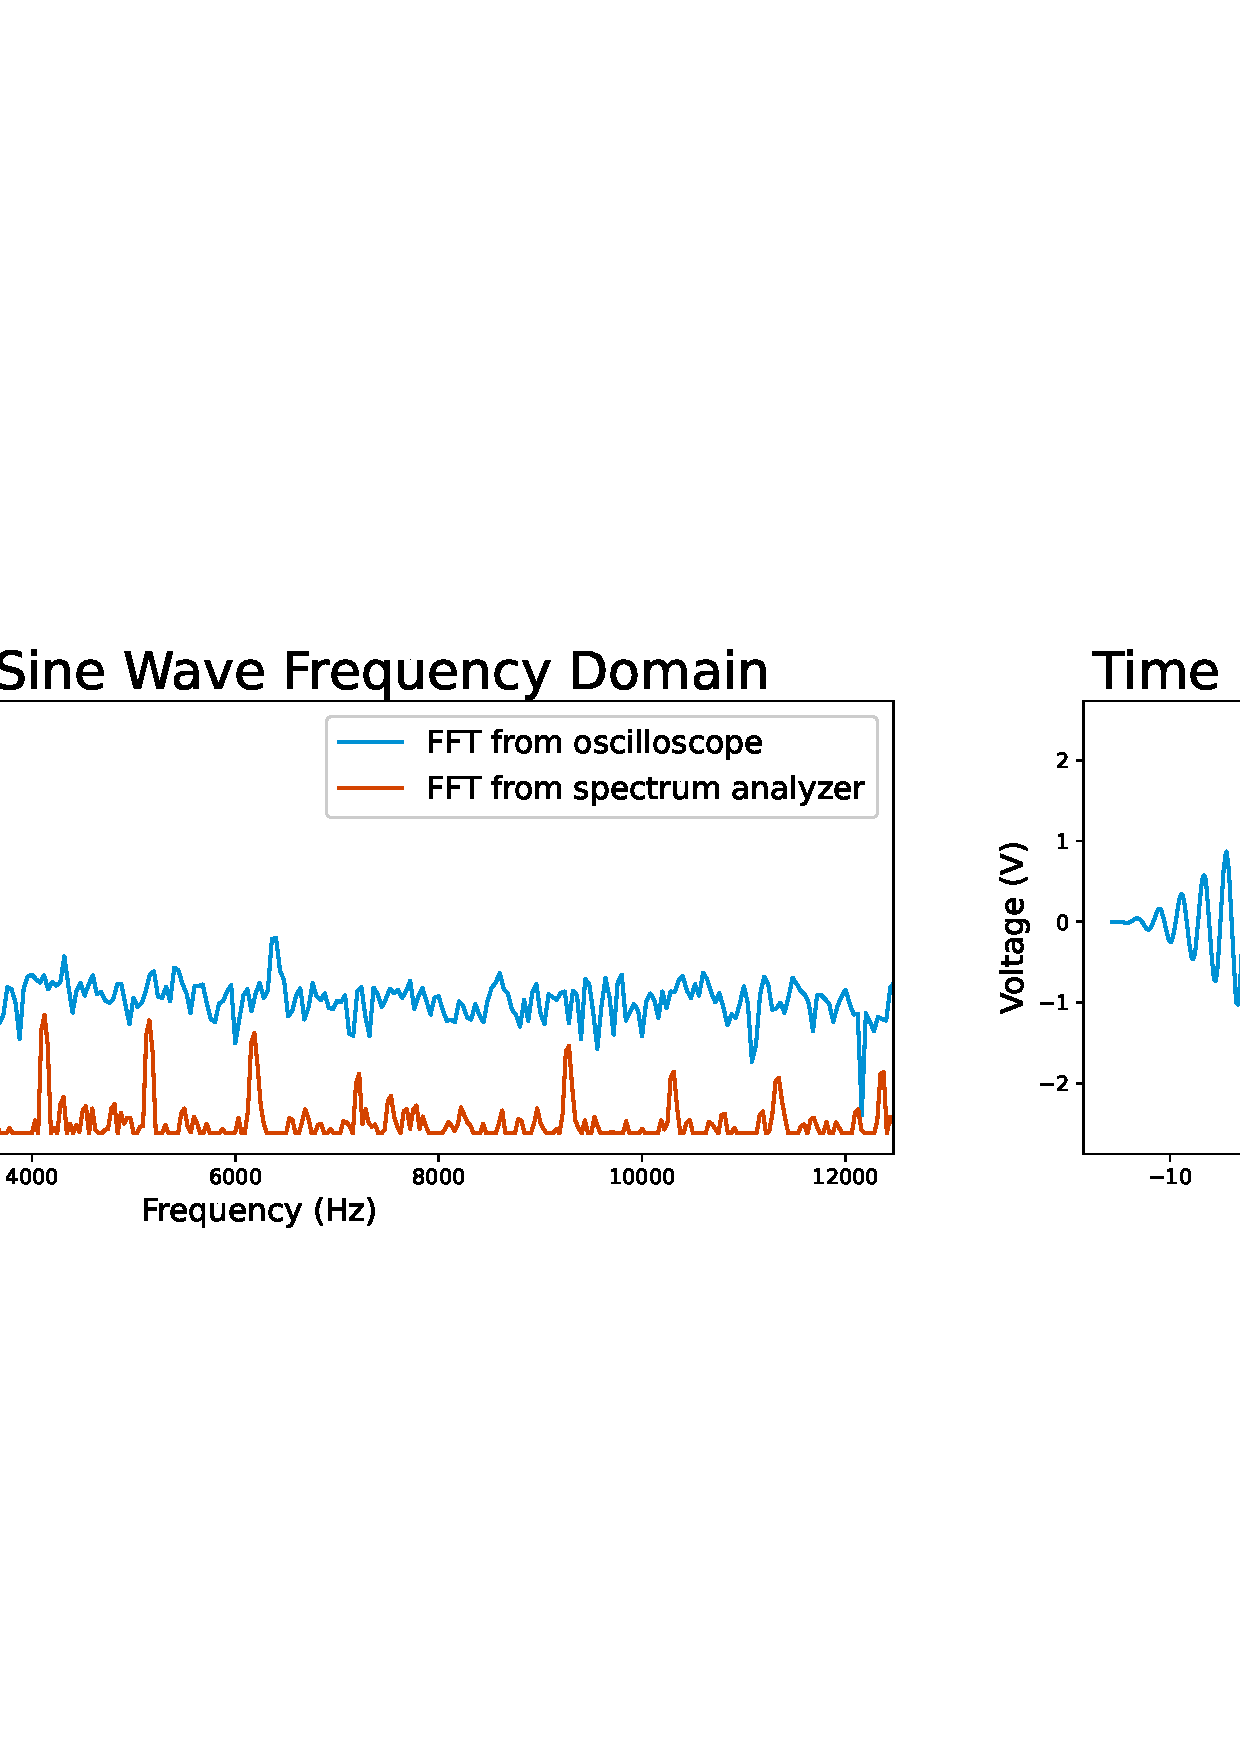
\includegraphics[width=\textwidth]{1_03 kHz Sine Wave (hanning)}
    \caption{FFT analysis of an inputted Sine wave, at 1kHz and 1.03kHz. The effect of the hanning window can be seen slightly disturbing the 1kHz wave, but dramatically improving the fit on the 1.03kHz wave. Notice for these graphs, and for all similar comparison graphs, the FFT from the Oscilloscope has been shifted to the right by 200Hz to help show the similarities in the graphs.}
    \label{fig:sine}
\end{figure} % Sine Waves  

\begin{figure}[!ht]
    \centering
    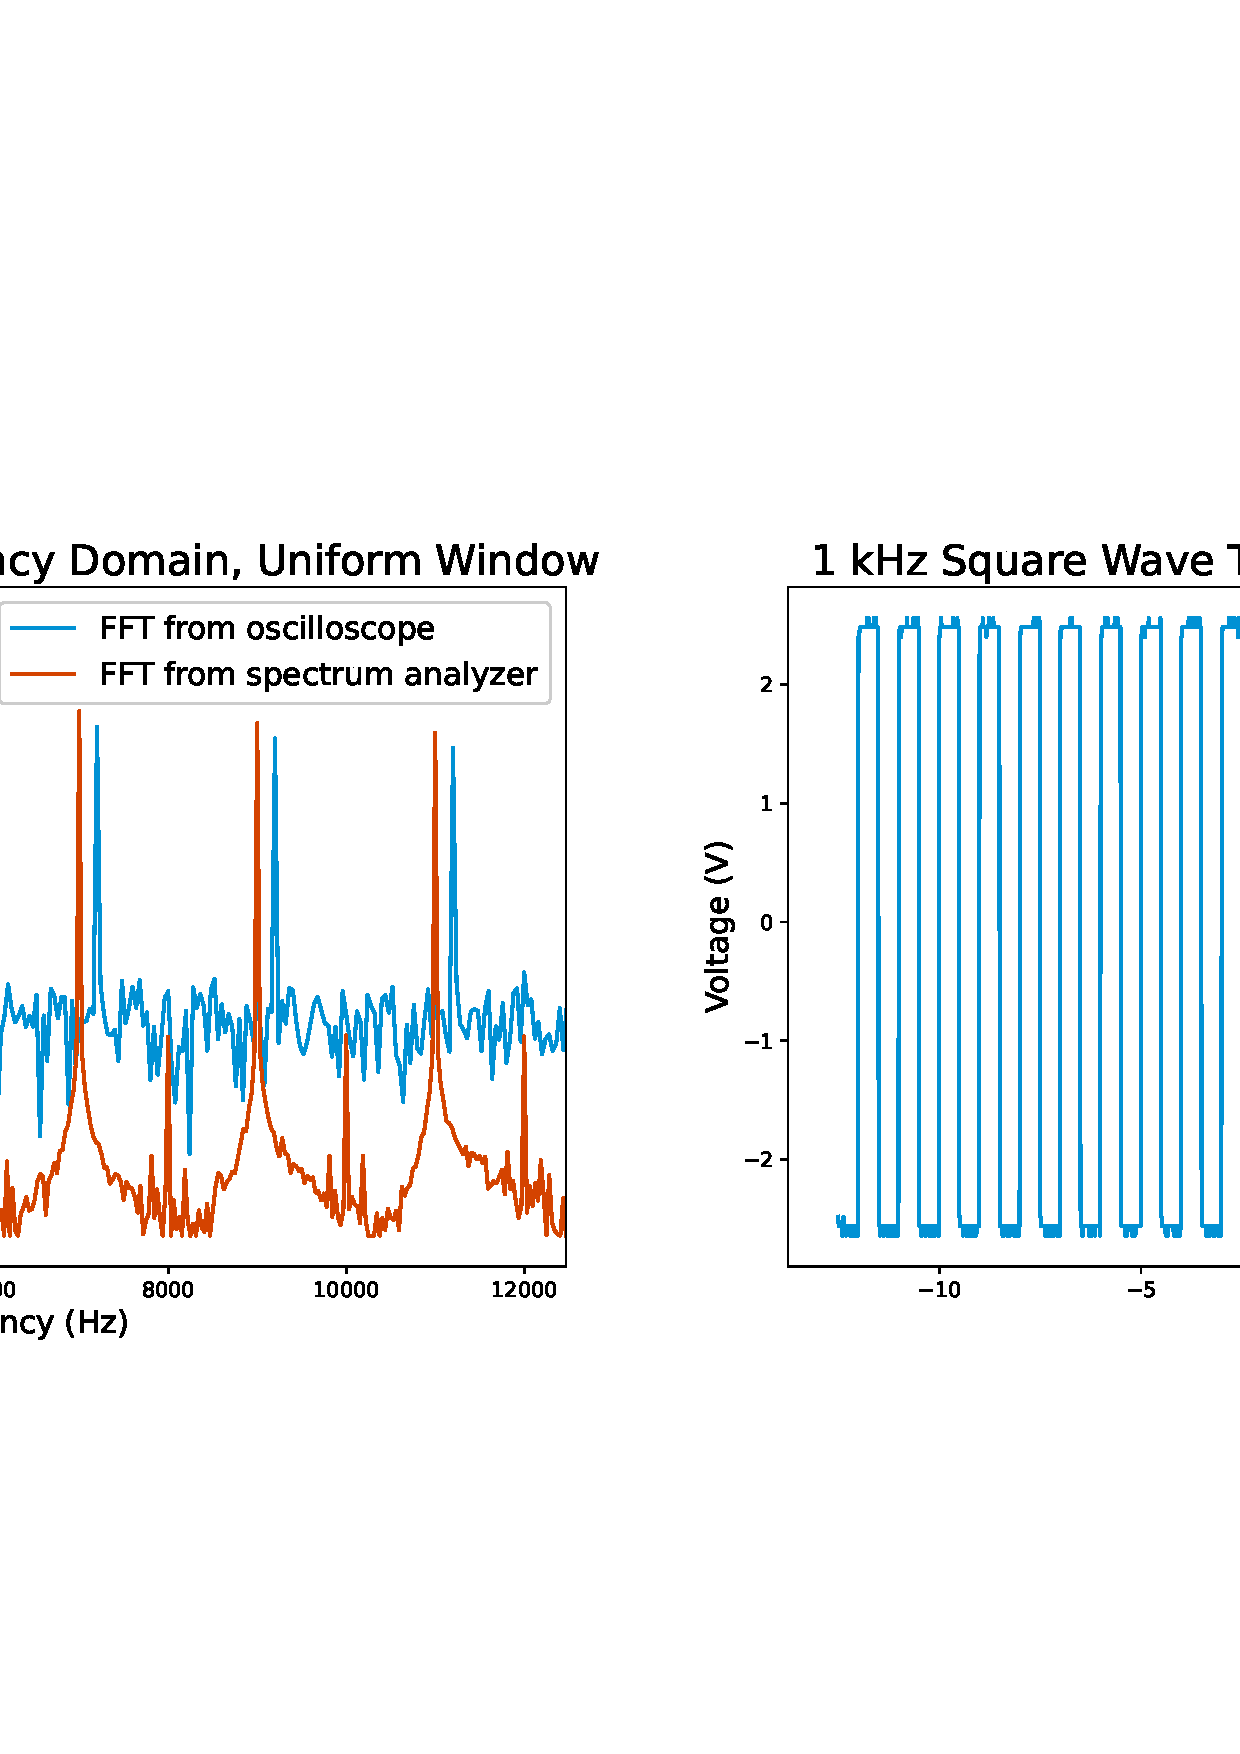
\includegraphics[width=\textwidth]{1 kHz Square Wave (uniform)}
    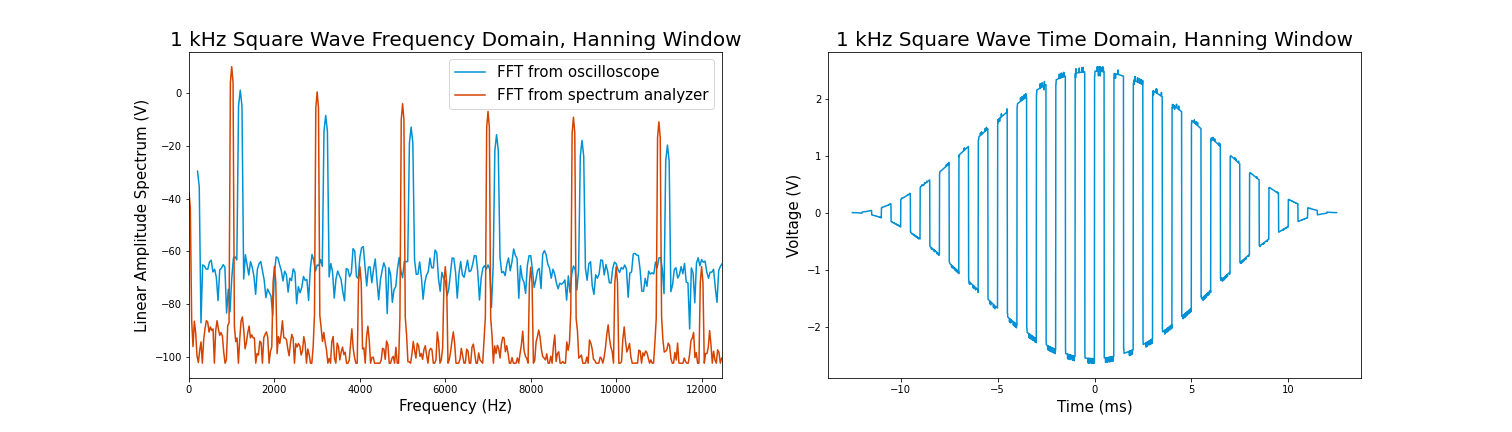
\includegraphics[width=\textwidth]{1 kHz Square Wave (hanning)}
    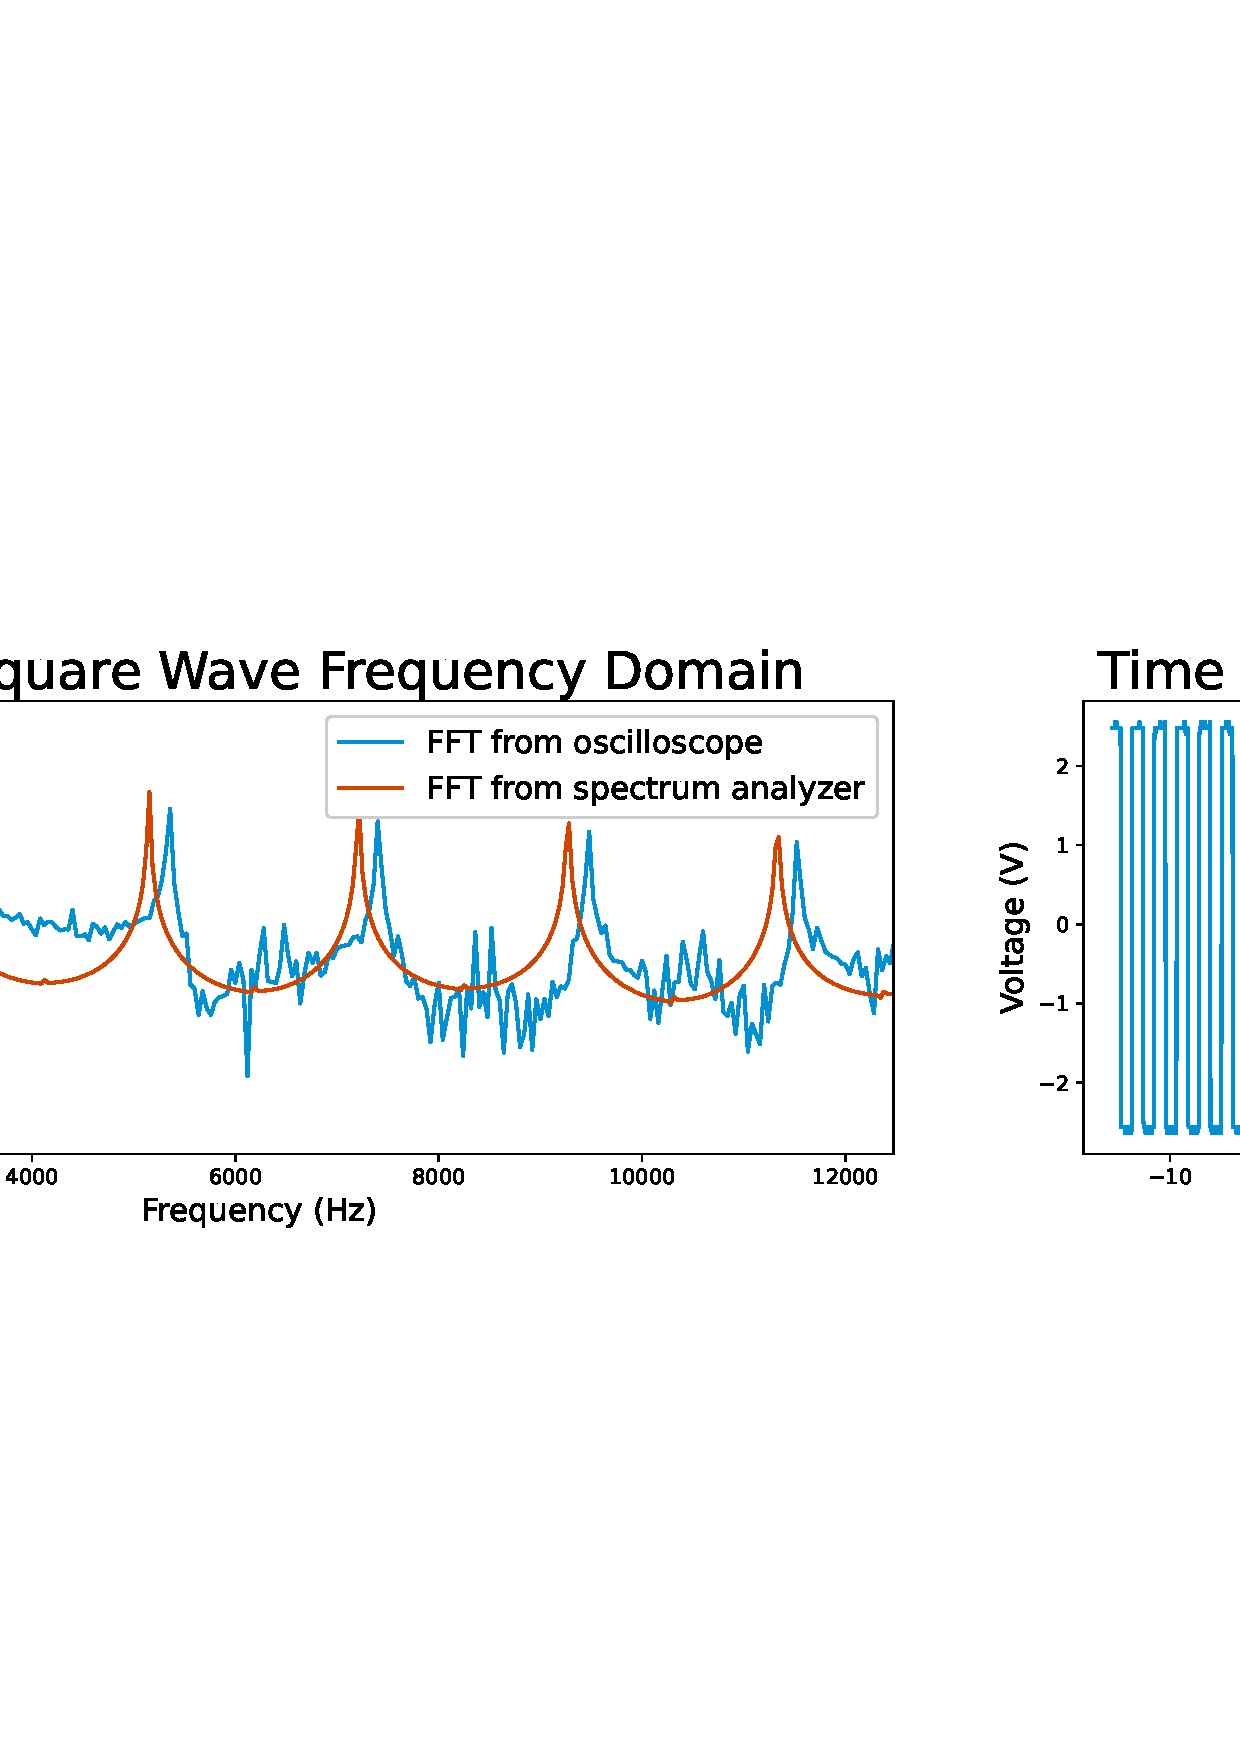
\includegraphics[width=\textwidth]{1_03 kHz Square Wave (uniform)}
    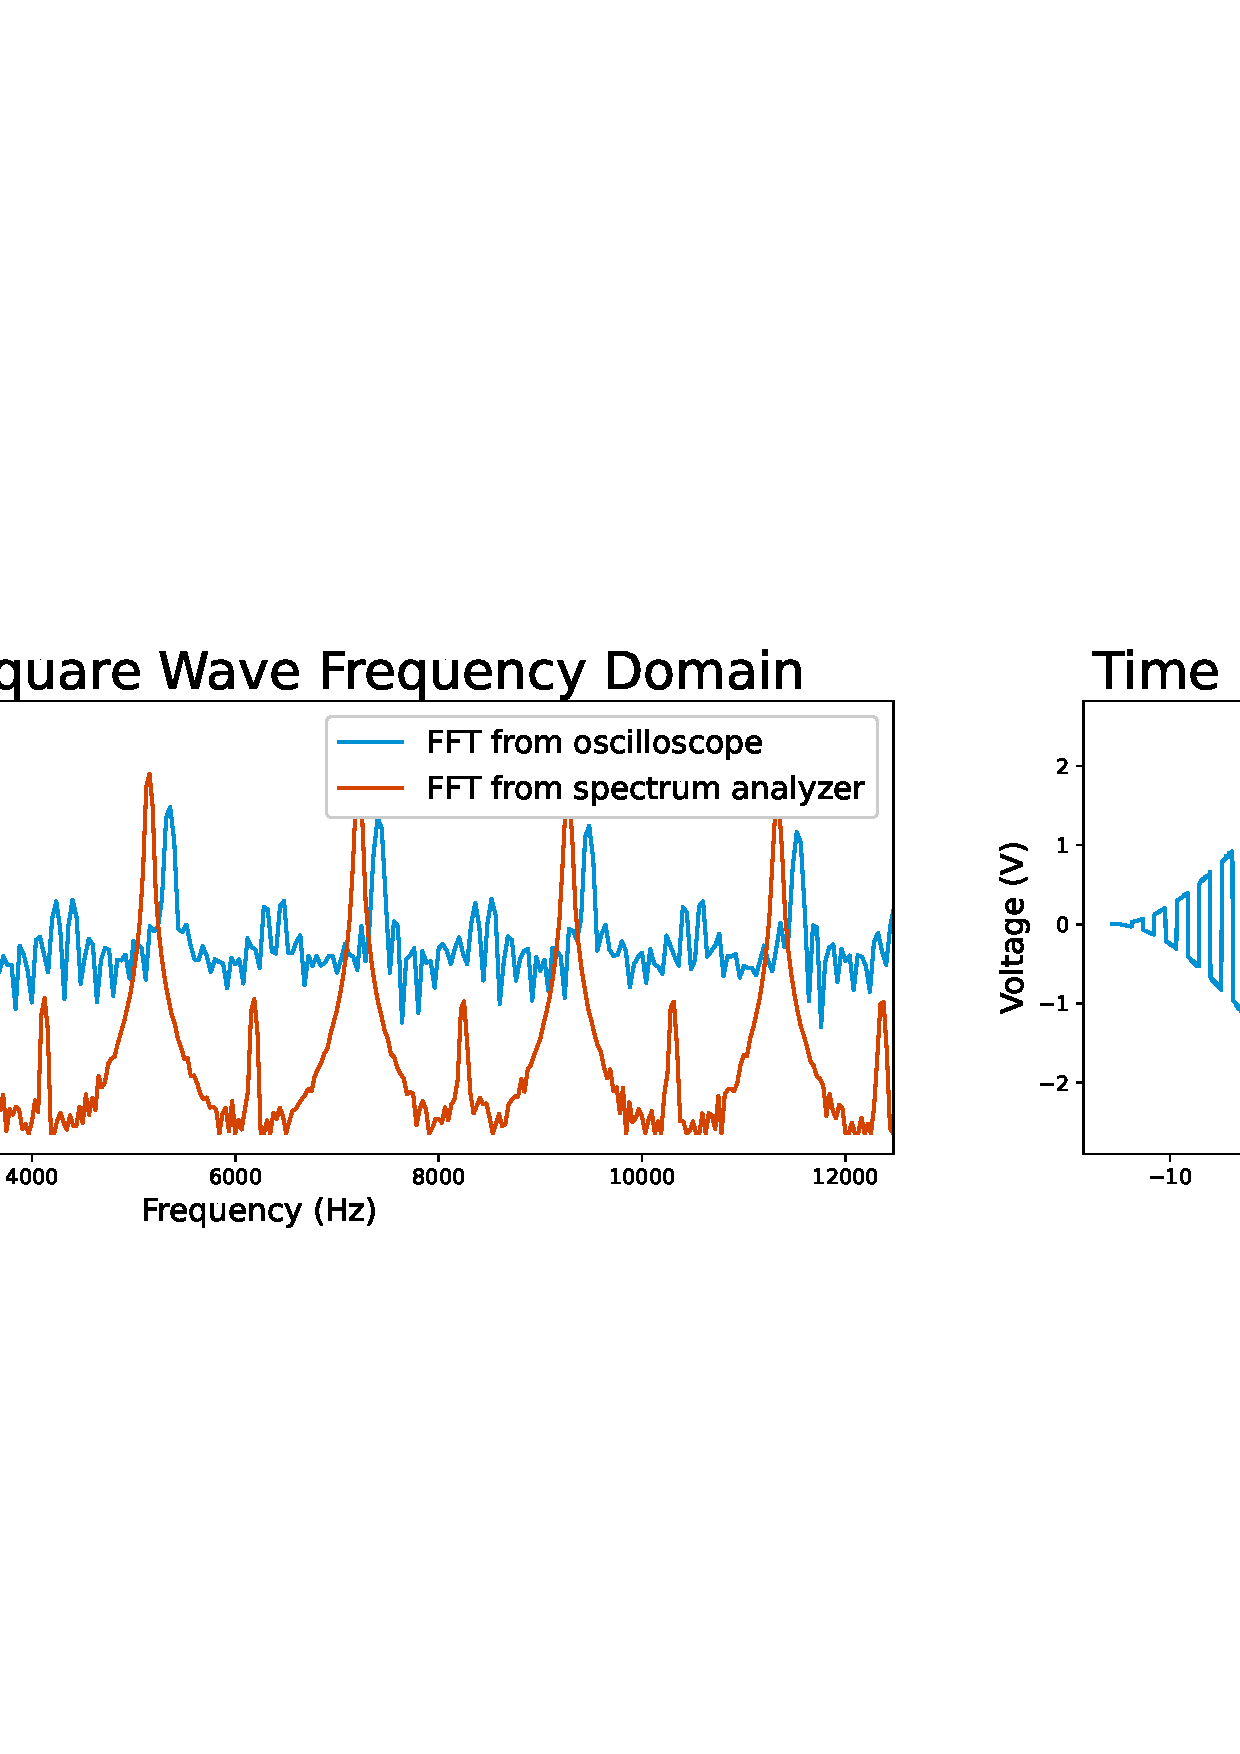
\includegraphics[width=\textwidth]{1_03 kHz Square Wave (hanning)}
	\caption{FFT analysis of an inputted square wave, at 1kHz and 1.03kHz. The effect of the hanning window can be seen slightly improving the 1kHz wave, but dramatically improving the fit on the 1.03kHz wave.}
    \label{fig:square}
\end{figure} % Square Waves

\begin{figure}[!ht]
    \centering
    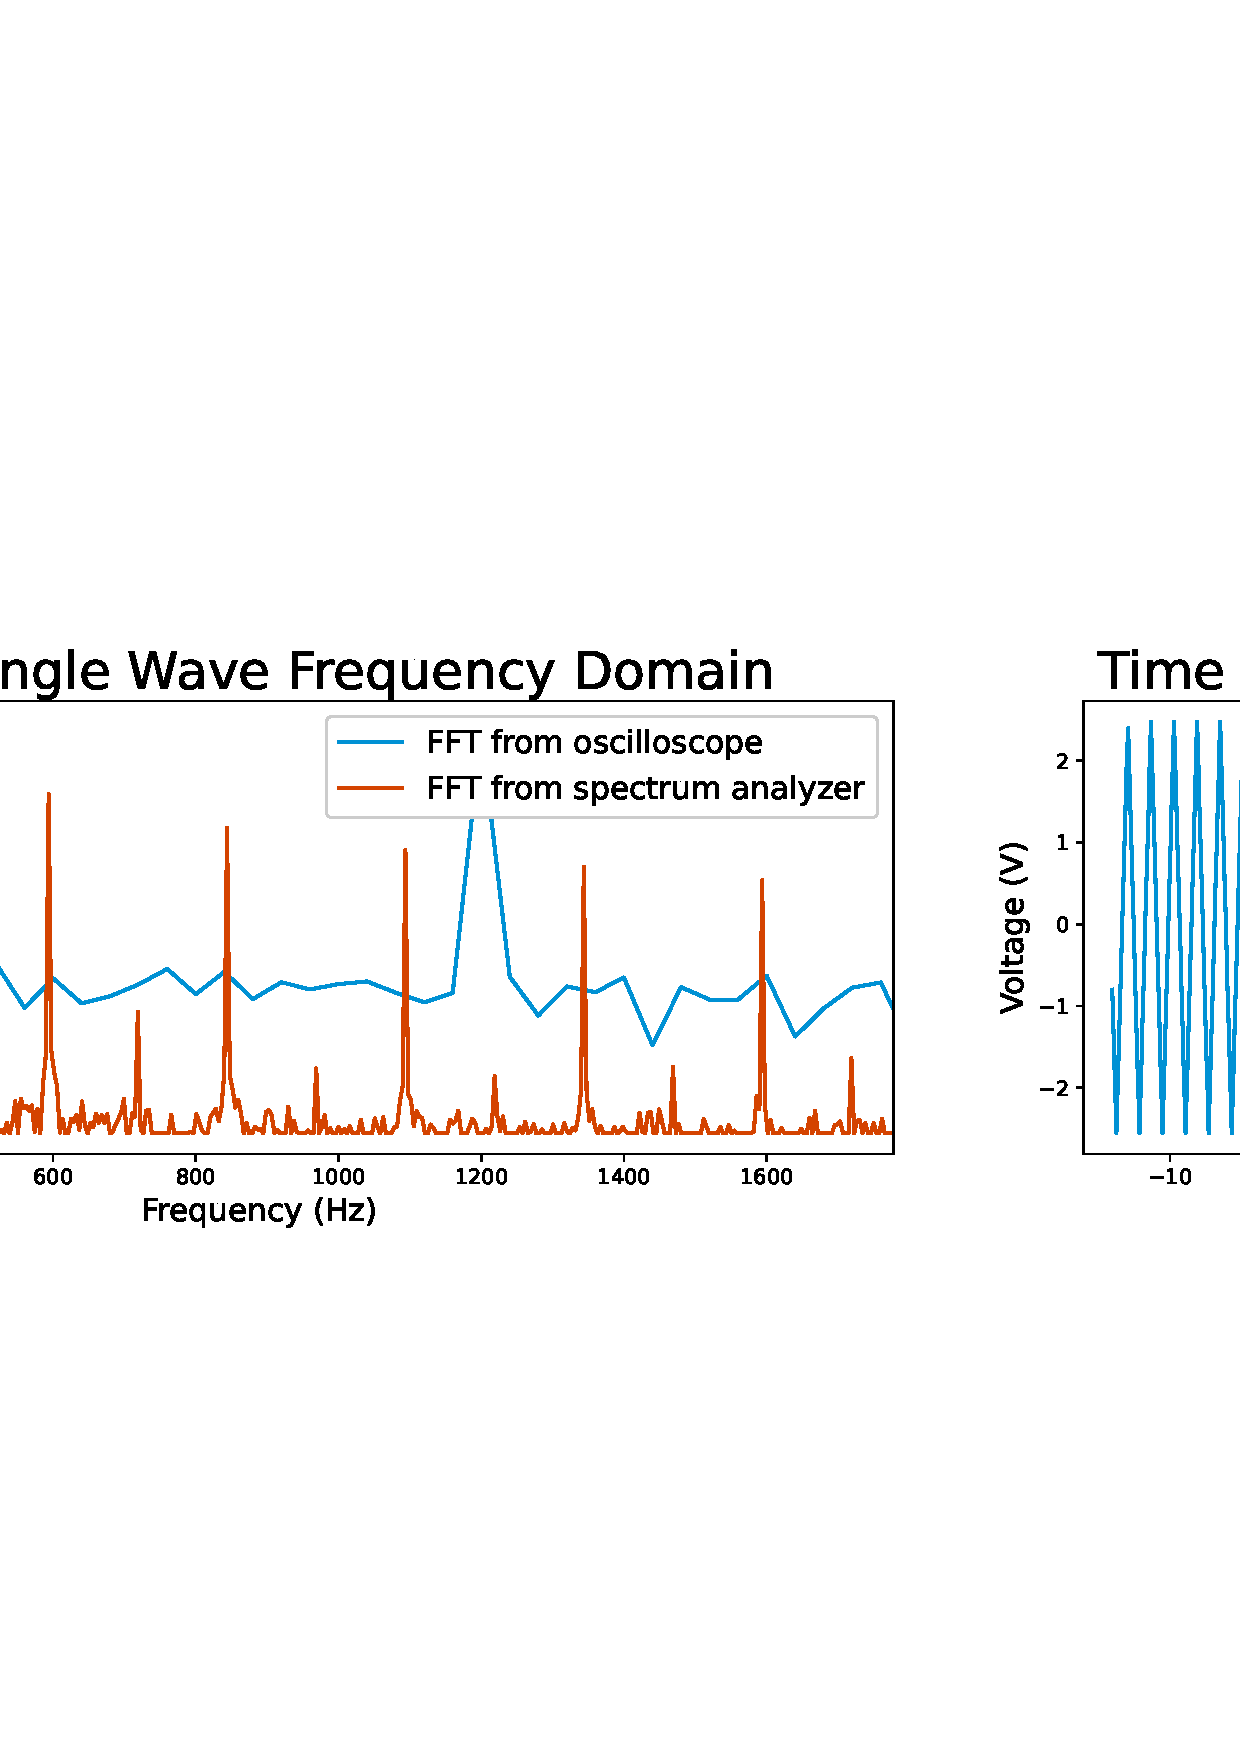
\includegraphics[width=\textwidth]{1 kHz Triangle Wave (uniform)}
    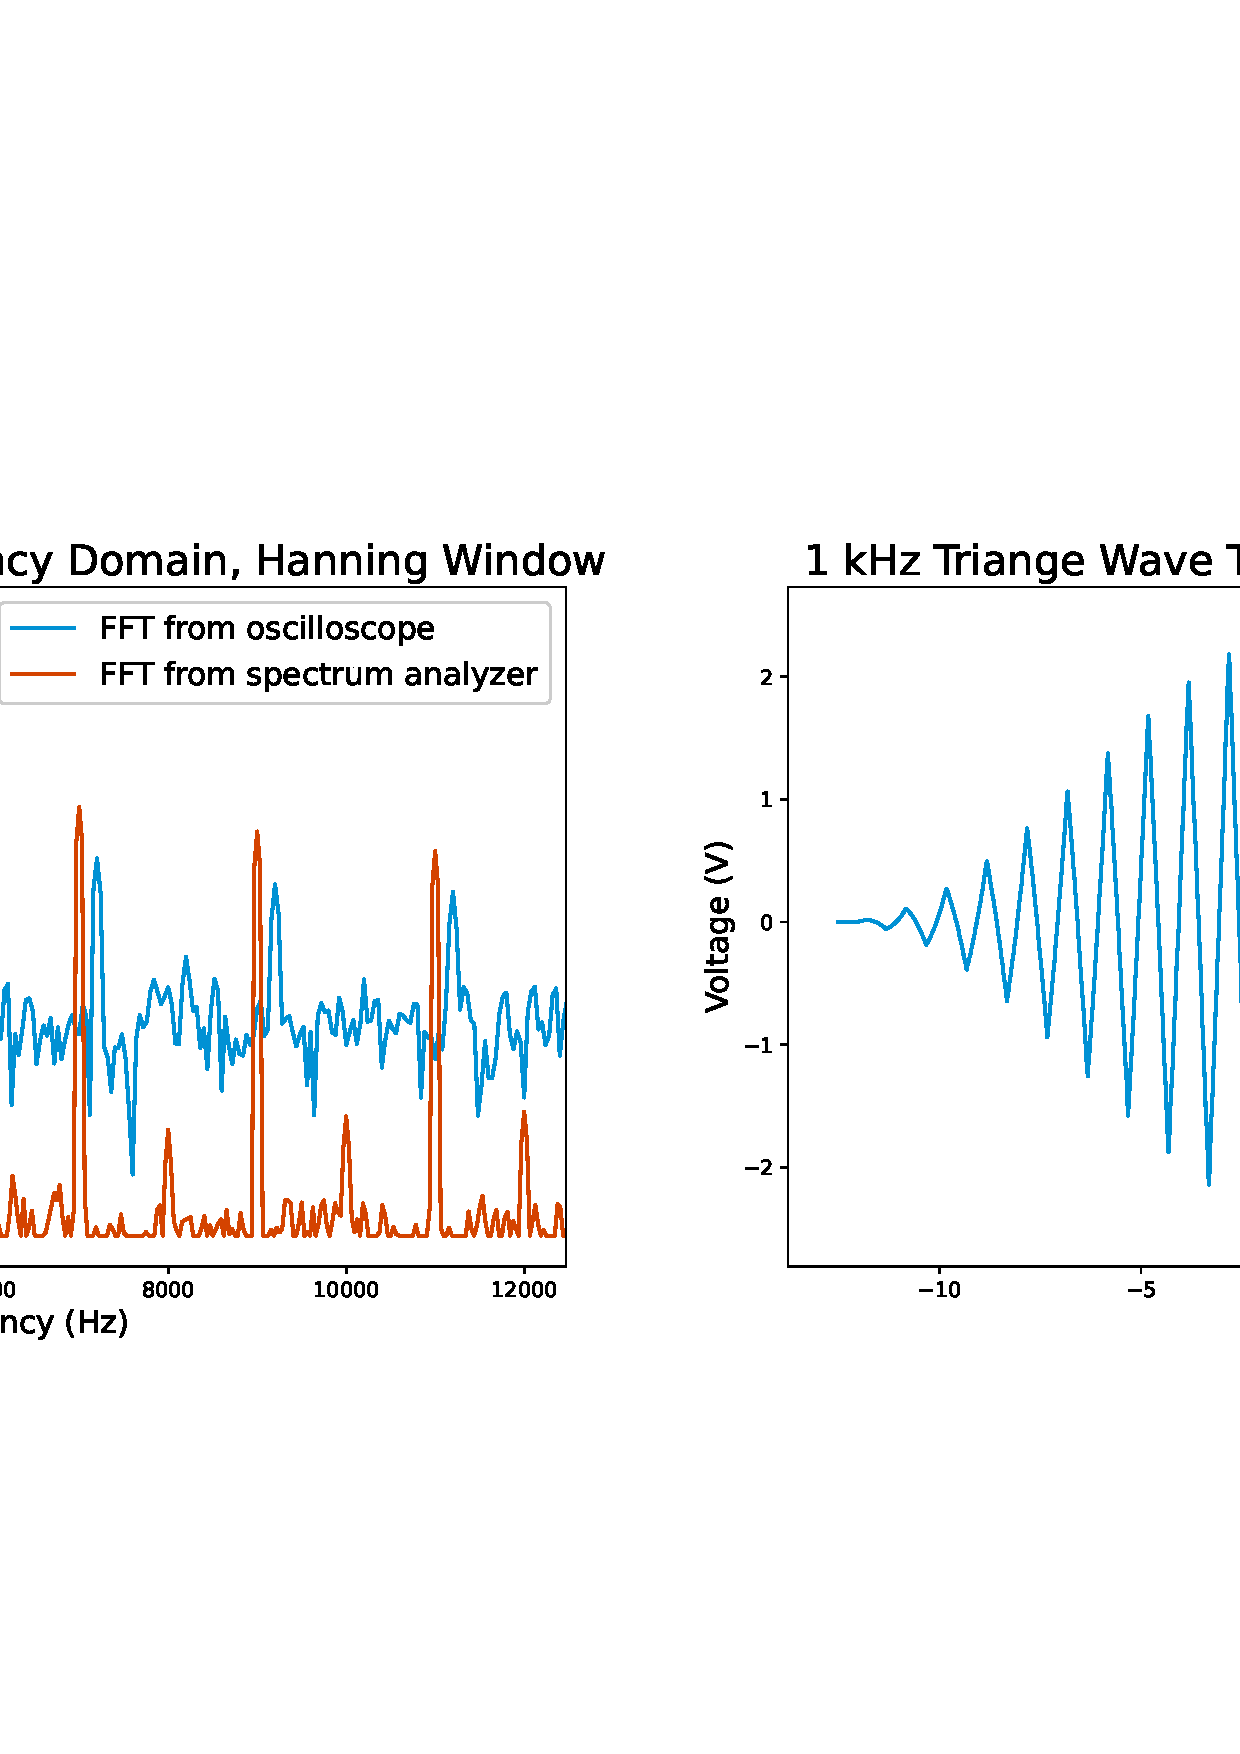
\includegraphics[width=\textwidth]{1 kHz Triange Wave (hanning)}
    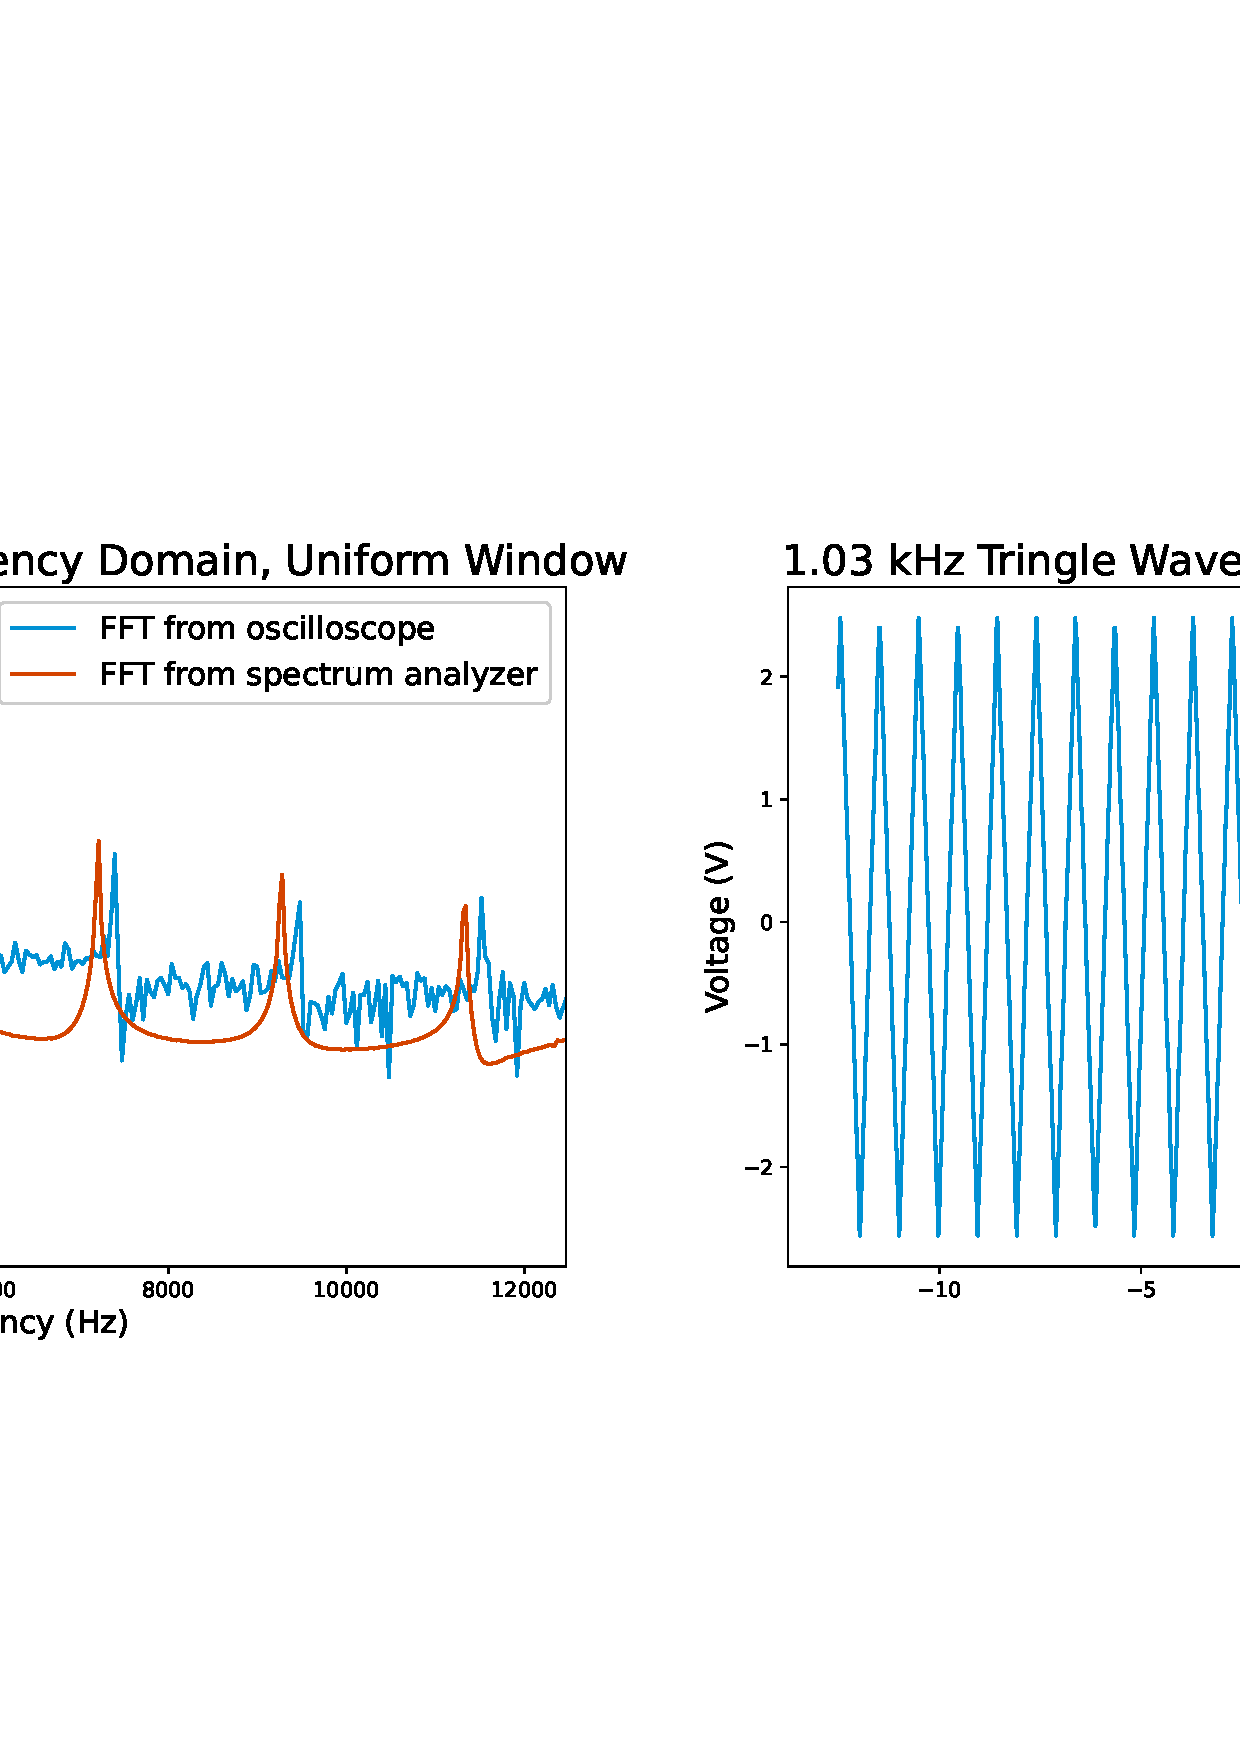
\includegraphics[width=\textwidth]{1_03 kHz Tringle Wave (uniform)}
    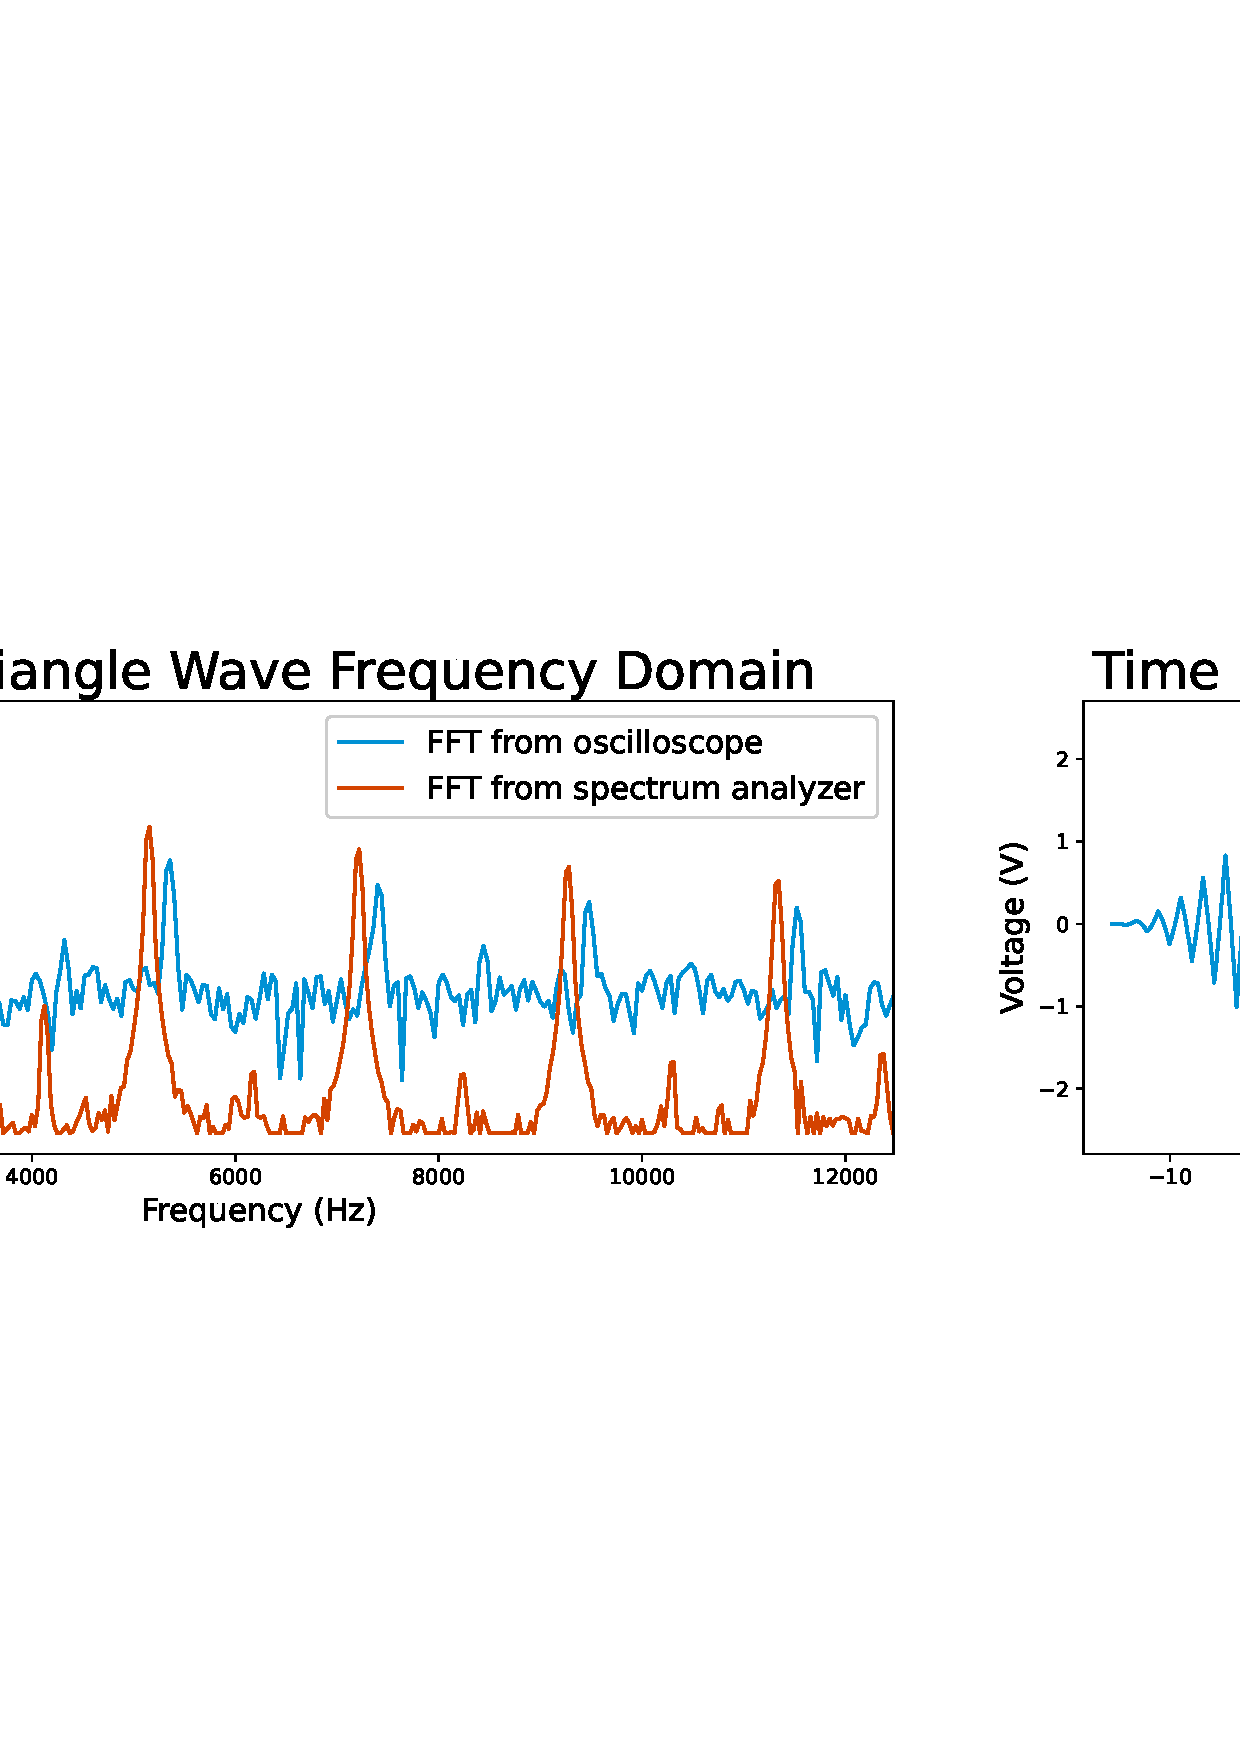
\includegraphics[width=\textwidth]{1_03 kHz Triangle Wave (hanning)}
    \caption{FFT analysis of an inputted triangle, or seesaw, wave, at 1kHz and 1.03kHz. The effect of the hanning window can be seen dramatically improve both the 1kHz and 1.03kHz waves. This graph gives the strongest demonstration of why the window function is better applied in a general setting.}
    \label{fig:triangle}
\end{figure} % Triangle Waves 

\begin{figure}[!ht]
    \centering
    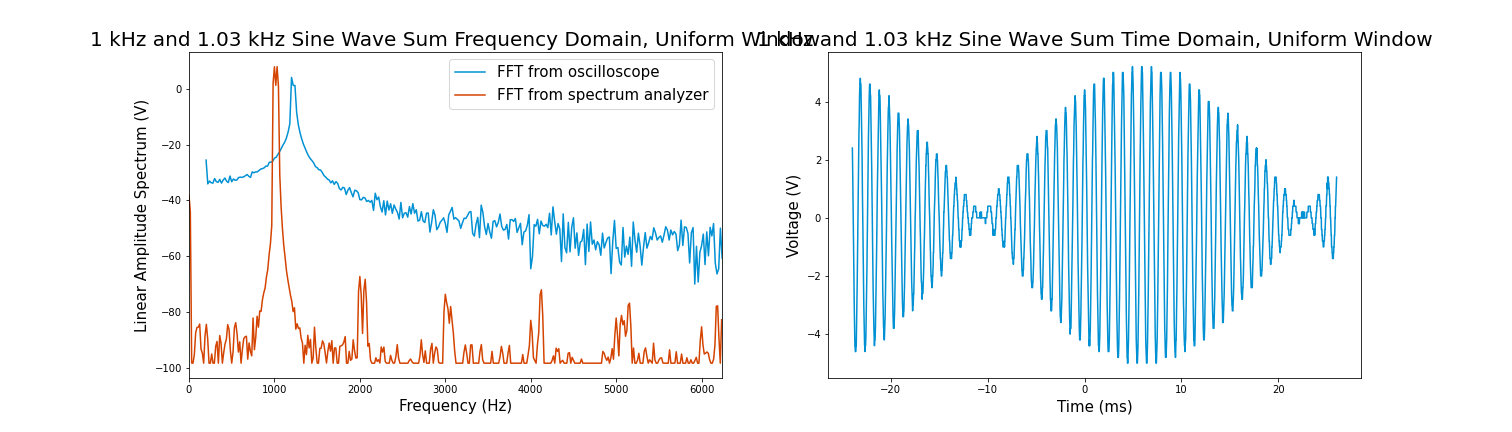
\includegraphics[width=\textwidth]{1 kHz and 1_03 kHz Sine Wave Sum (uniform)}
    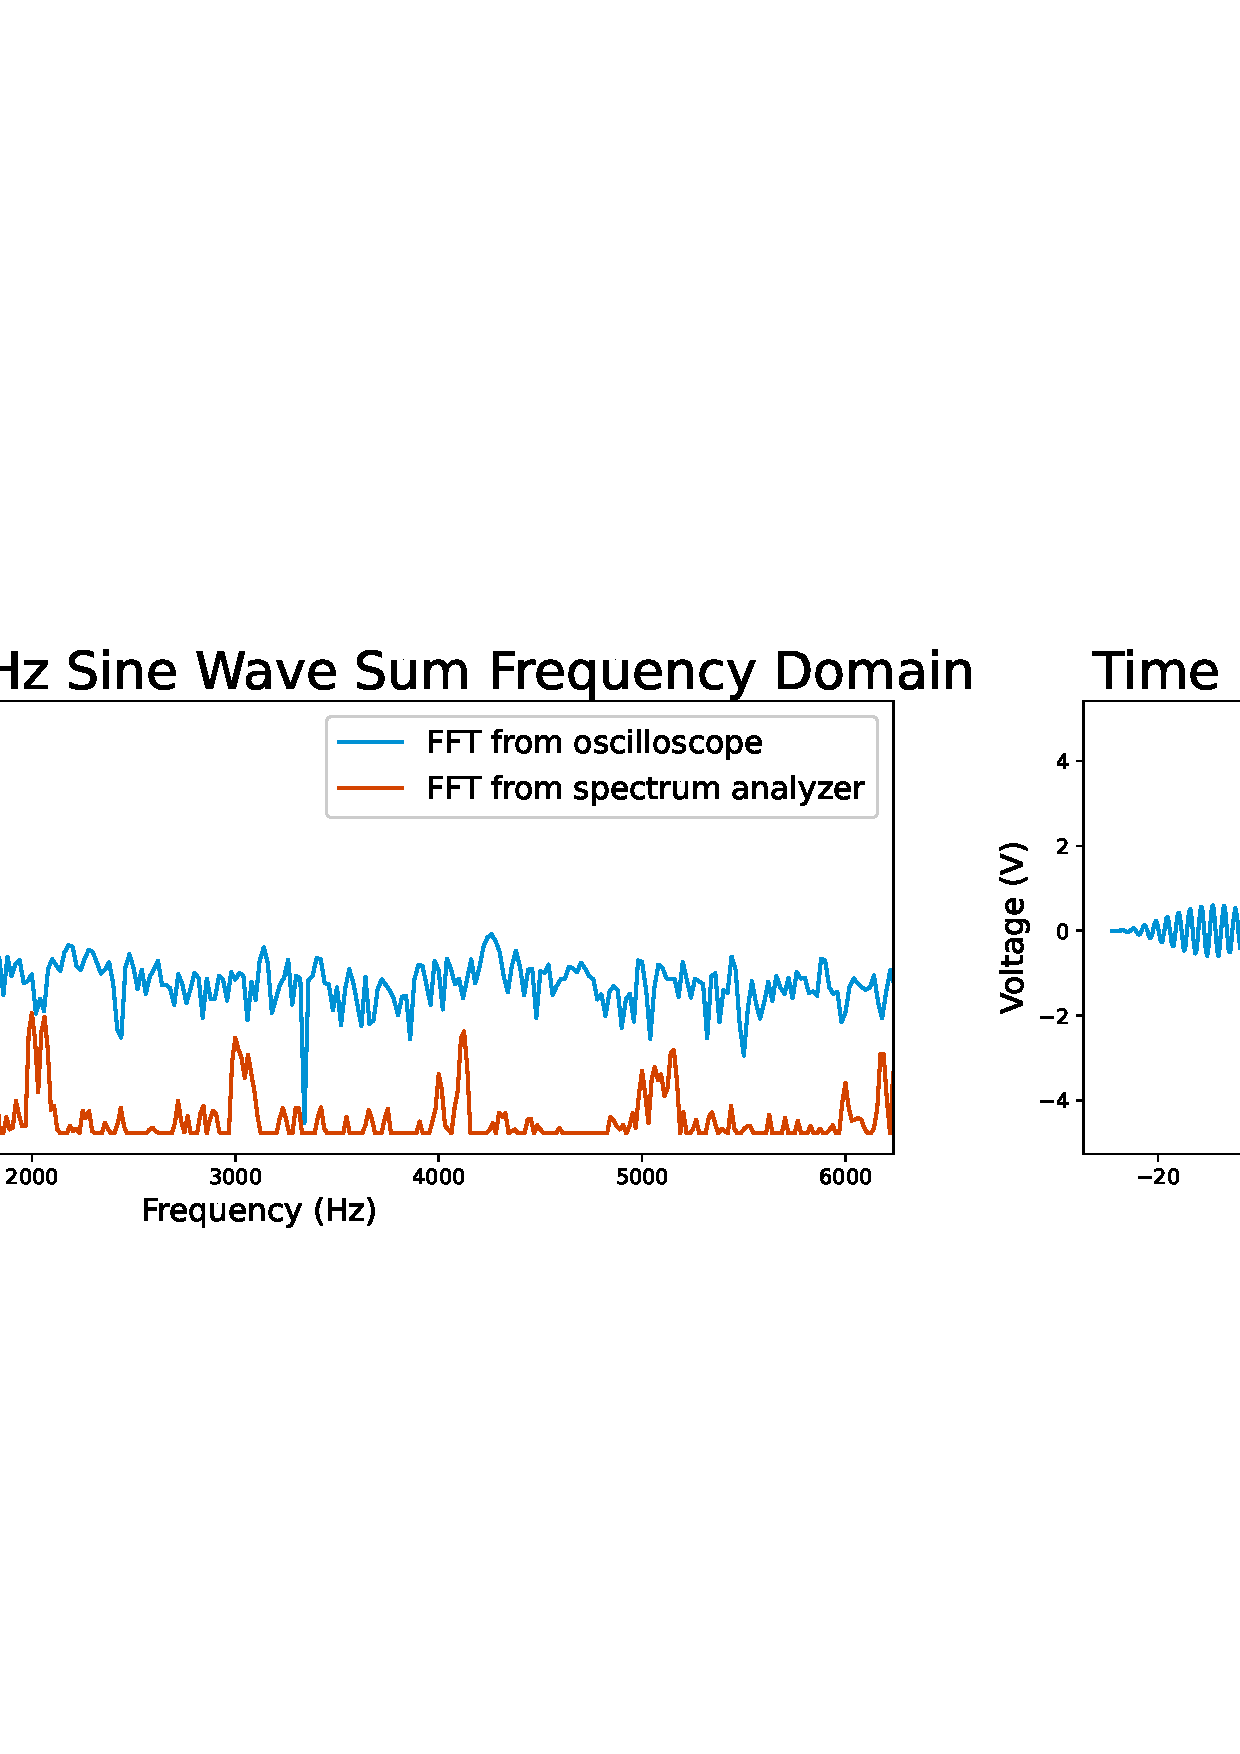
\includegraphics[width=\textwidth]{1 kHz and 1_03 kHz Sine Wave Sum (hanning)}
    \caption{FFT analysis of a sum of a 1kHz and 1.03kHz Sine wave.}
    \label{fig:sine_sum}
\end{figure} % sum
    
\begin{figure}[!ht]
    \centering
    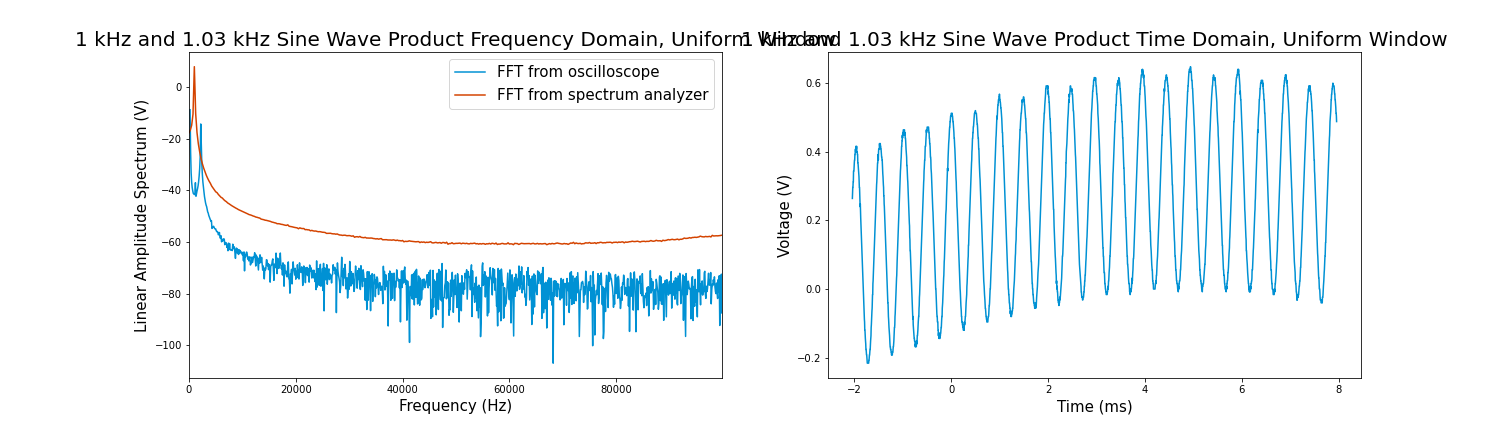
\includegraphics[width=\textwidth]{1 kHz and 1_03 kHz Sine Wave Product (uniform)}
    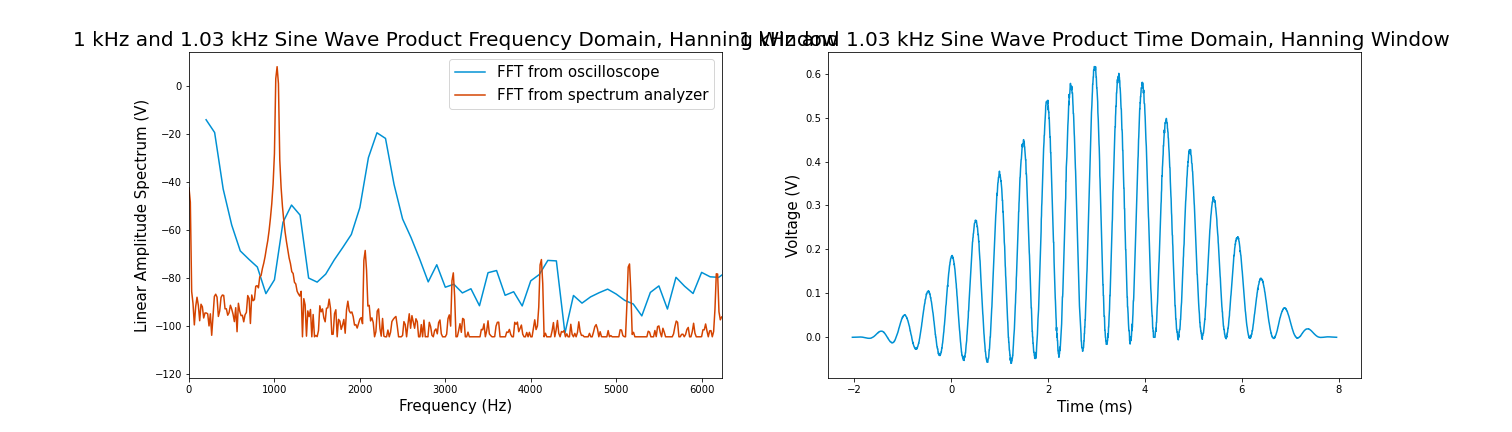
\includegraphics[width=\textwidth]{1 kHz and 1_03 kHz Sine Wave Product (hanning)}
    \caption{FFT analysis of a product of a 1kHz and 1.03kHz Sine wave.}
    \label{fig:sine_product}
\end{figure} % product
    
\begin{figure}
\centering
    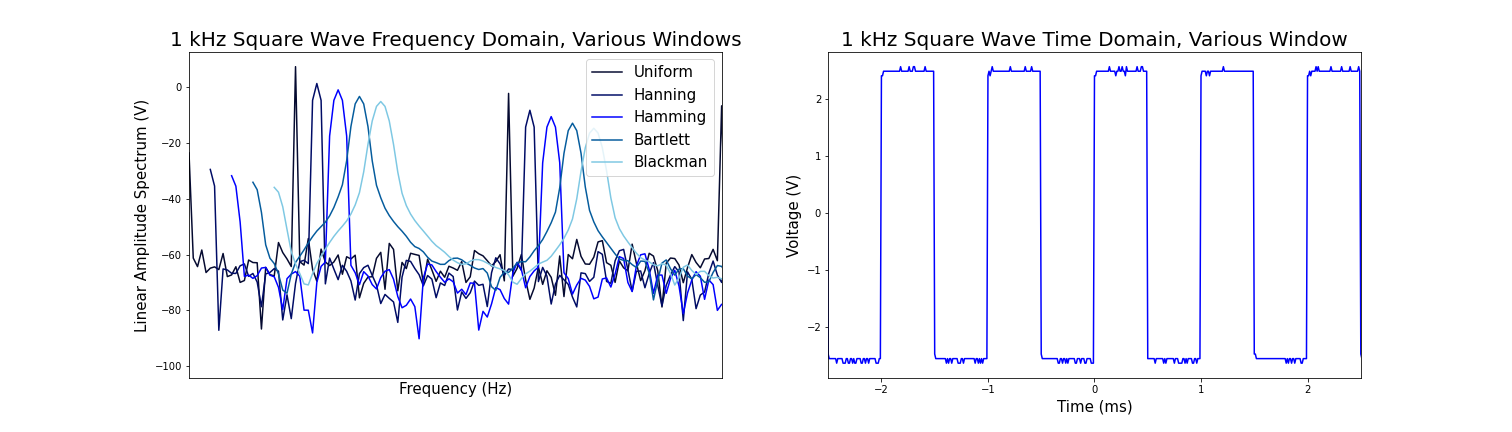
\includegraphics[width=\textwidth]{Variety of Windows}
	\caption{FFT analysis of a 1kHz triangle wave with various applied window functions. It seems that the uniform window has the worst results, while the going down the list seems widen the possible results of the analysis. Each FFT has been shifted on the right and the frequency-axis omitted to prevent misunderstanding.}
    \label{fig:various_windows}
\end{figure} % variety of windows 

\begin{figure}[!ht]
    \centering
    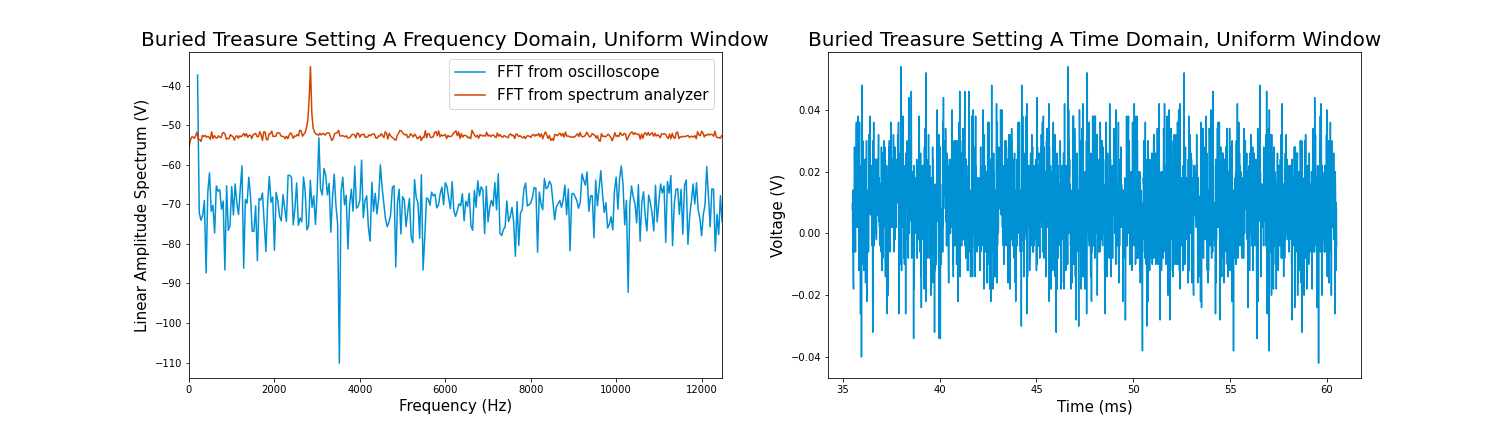
\includegraphics[width=\textwidth]{Buried Treasure Setting A (uniform)}
    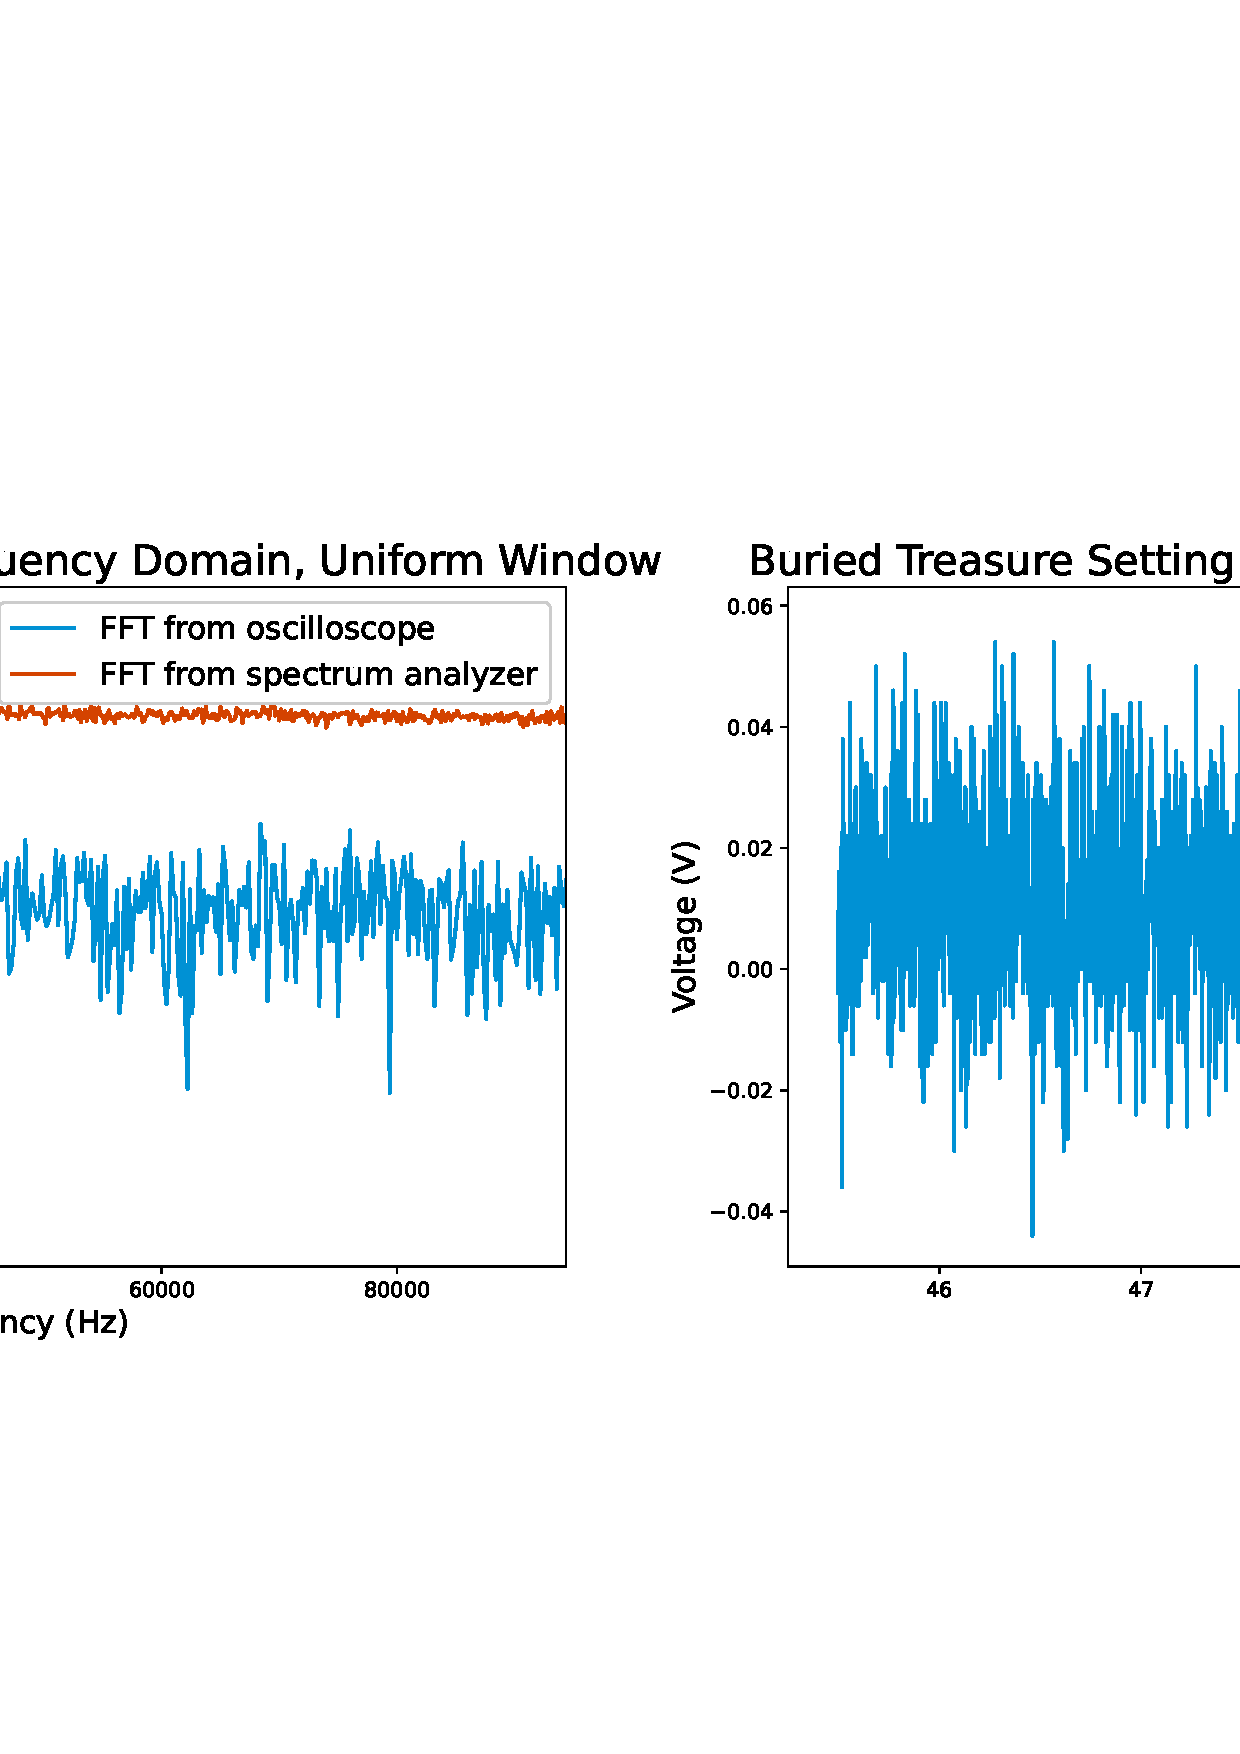
\includegraphics[width=\textwidth]{Buried Treasure Setting B (uniform)}
    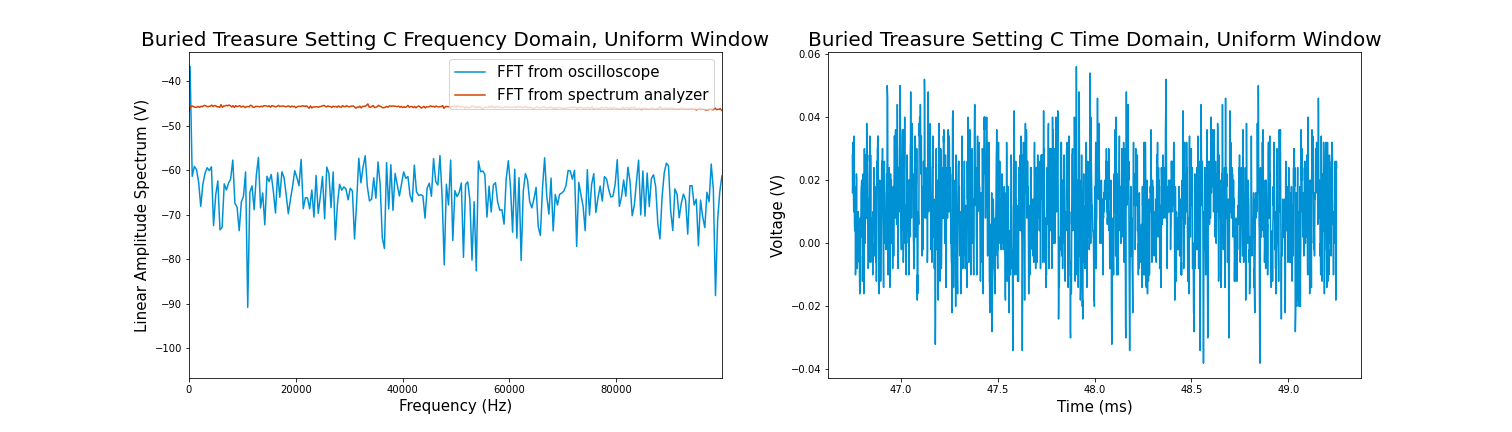
\includegraphics[width=\textwidth]{Buried Treasure Setting C (uniform)}
    \caption{The FFT analysis for the provided Buried Treasure module. Setting A has an easy to see peak at around 3kHz, however the time domain did not have enough averaging to see a definitive peak in that data. Similarly, neither the spectrum analyzer or the oscilloscope were averaged over long enough to see the buried Sine wave on settings B or C.}
    \label{fig:buried}
\end{figure} % buried treasure   
    
%% Results and Analysis section. Here I go into what we actually got out of the tests and the resulting calculations from them. 
\section{Results and Analysis}
    
This lab has been split up into the three different stages as explained above. The first outlines the first experiences with the spectrum analyzer and manually applying the FFT to the time domain in order to achieve the expected results. The second part goes over the LRC response function. The third goes over the acoustical cavity response function. 
    

    
\subsection{General Fourier Introduction}
It can be seen that the difference between the uniform window and hanning window applied on the 1kHz wave isn't very noticeable (Figure~\ref{fig:sine}). However, when applied to a frequency that wasn't as ideal, the hanning correction made the FFT of the 1.03kHz frequency look comparable to that of the 1kHz frequency (Figure~\ref{fig:sine}). It seems that using the hanning window on anything, other than the ideal Sine Wave, returned a more reasonable analysis; for both the spectrum analyzer and the oscilloscope. This general idea held for testing a square wave (Figure~\ref{fig:square}) and the triangle, or seesaw, wave (Figure~\ref{fig:triangle}). It can be seen that the FFT of the less ideal frequency has a wider spread of possible frequency peak. This should serve as the practical average and standard deviation of the result; taking the highest peak as the average and the HMFW to be the standard deviation.
    
To test the impact of different windows on the FFT, five different windows were tested on a square wave (Figure~\ref{fig:various_windows}). While this doesn't give any enlightenment as to where each shines, the largest take away is that the four window functions that are not the uniform window effectively grounded the noise introduced to the FFT by a non-periodic function.  
    
The final test to see if we understood Fourier Analysis was to find the treasure buried in the noise provided. The tests were labeled A, B, C, and D. The first three were attempted, and only the first two could be found within the time restraint. On setting A, once the data was averaged over a large number of passes, about 1000, the spectrum analyzer seemed to give a definitive spike (Figure~\ref{fig:buried}). The oscilloscope collected data with an acquire time about the same as that used for the spectrum analyzer, 32ms, and averaged over 128 passes. Even with the large amount of data collection, the peak is barely visible. On setting B (Figure~\ref{fig:buried}), with even more passes averaged and an acquire time of 8ms, the spectrum analyzer could barely pick out the peak and nothing was found from the FFT done post lab. On setting C (Figure~\ref{fig:buried}), the noise was so dominant nothing was able to be picked out. 

\subsection{LRC Analysis}
 
 \begin{figure}[!ht]
\centering
    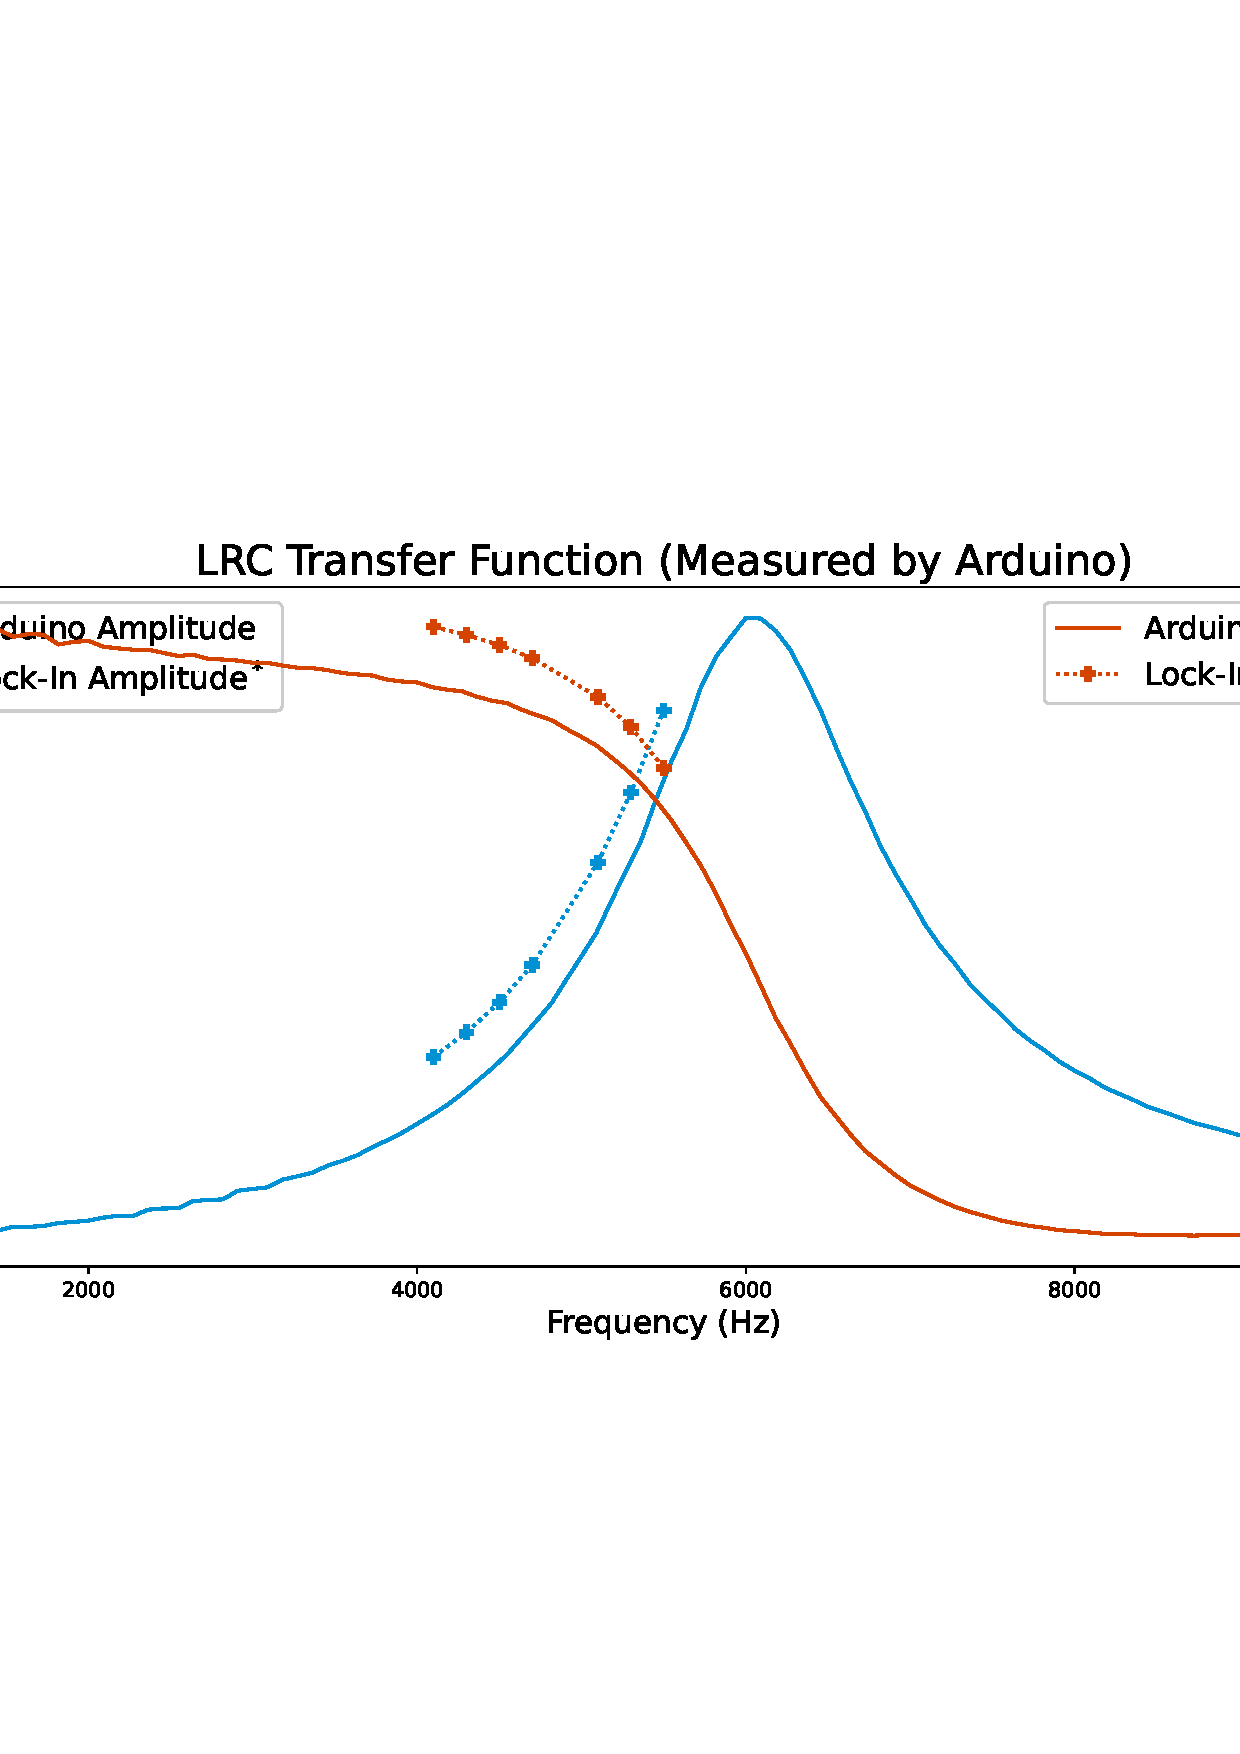
\includegraphics[width=\textwidth]{arduino data_}
    \caption{Analysis of amplitude and phase shift from Arduino and Lock-In Amplifier. For some reason, the amplitude given by the Lock-In Amplitude needed to be decreased by a factor of 3.5 to be comparable. The qualitative results still hold.}
    \label{fig:LRC_Arduino}
\end{figure} % LRC Arduino 

   
\begin{figure}[!ht]
\centering
    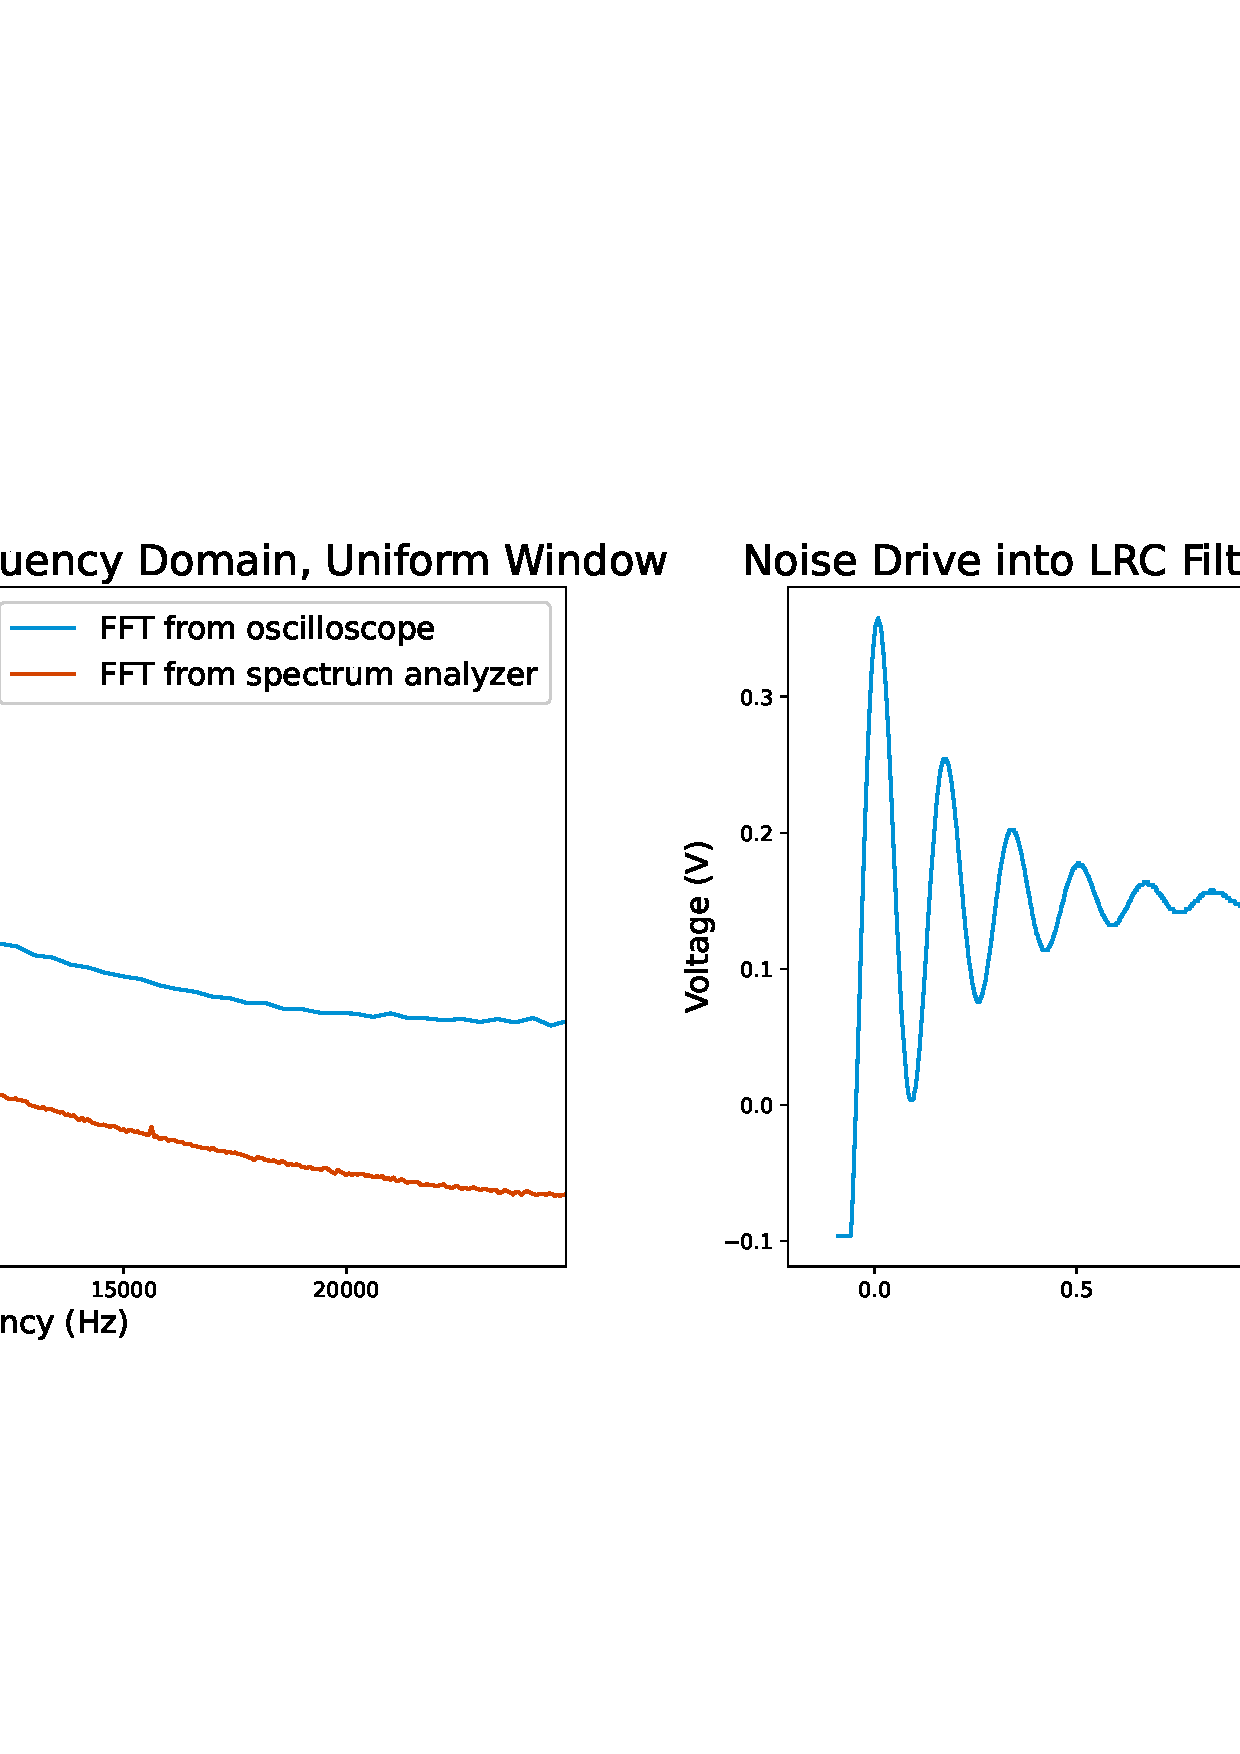
\includegraphics[width=\textwidth]{Noise Drive into LRC Filter (uniform)}
    \caption{FFT analysis of noise drive into LRC circuit. the analysis has been done with a uniform window.}
    \label{fig:LRC_fft}
\end{figure} % LRC FFT
       
    
Analyzing the LRC circuit turned out to be more successful, as most of the tribulation of learning how to use the oscilloscope and spectrum analyzer were subsided. Analyzing the plots in Figures~\ref{fig:LRC_fft}, the max height is reached at a frequency of 6062.5Hz for the spectrum analyzer and a frequency of 6000Hz for the oscilloscope. These numbers are in good agreement with each other. From the Arduino data, the max amplitude was reached at a frequency of 6000Hz and the phase shift was $-90^\circ$ at 6091Hz. The lock-in amplifier can be seen to have the same trend as the Arduino in Figure~\ref{fig:LRC_Arduino}; however, not enough data was taken to see the where the maximum was. So, disregarding the lock-in data, all four graphs have good agreement.

The equations in Eq~\ref{eq:LRC} don't have enough degrees of freedom to discern the capacitance and inductance from this measurement. However, the product can be measured:
\[LC = \frac{1}{\sqrt{6000}}\approx 0.0129 \, \text{s}\]
    
    
\begin{figure}[!ht]
    \centering
    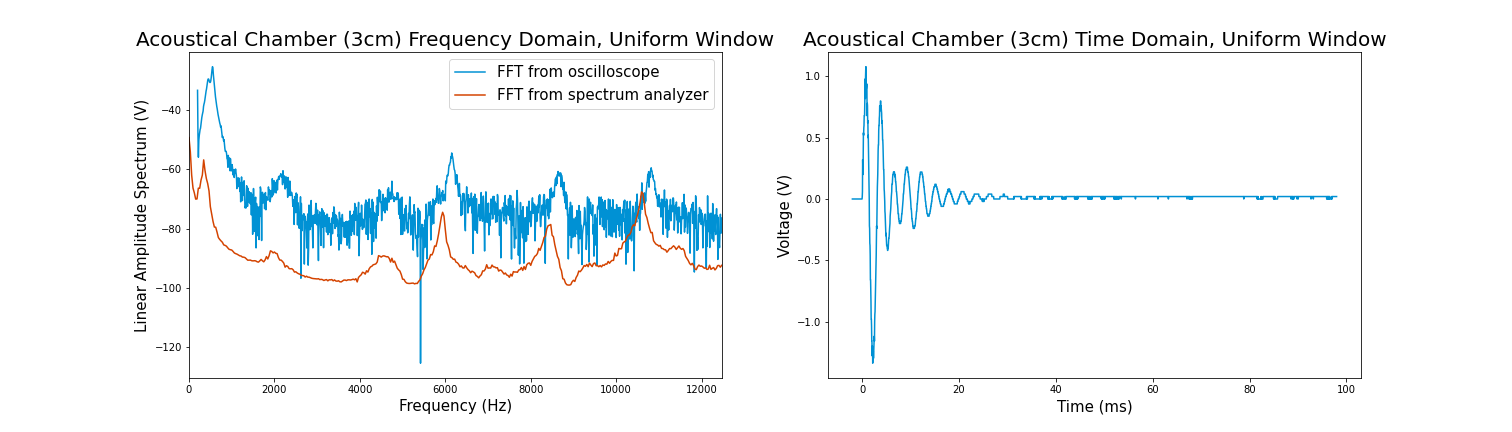
\includegraphics[width=\textwidth]{Acoustical Chamber (3cm) (uniform)}
    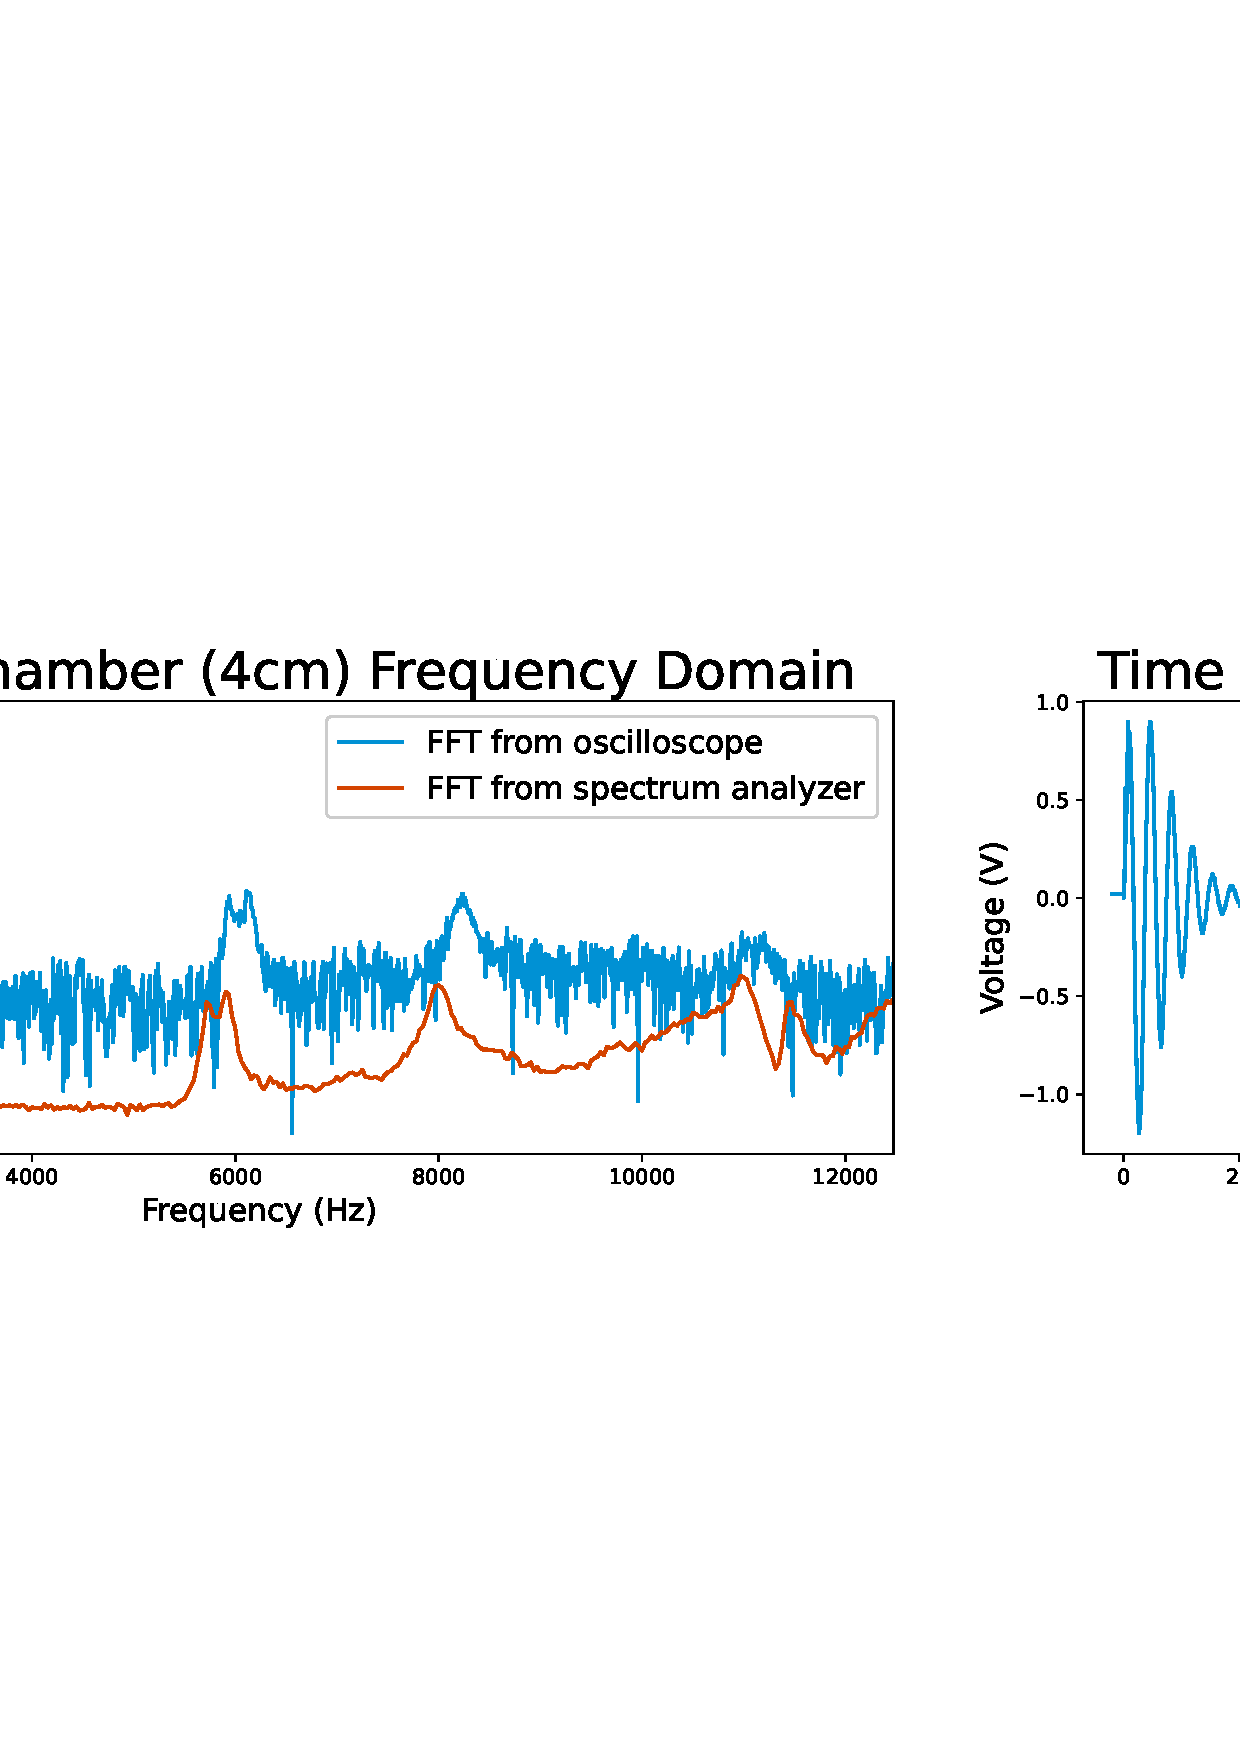
\includegraphics[width=\textwidth]{Acoustical Chamber (4cm) (uniform)}
    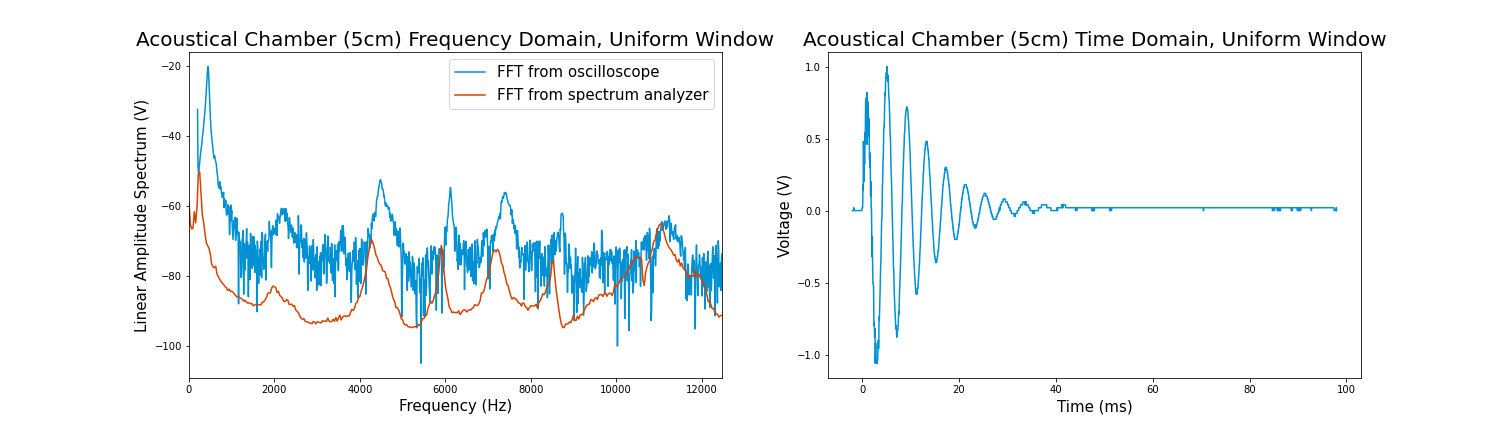
\includegraphics[width=\textwidth]{Acoustical Chamber (5cm) (uniform)}
    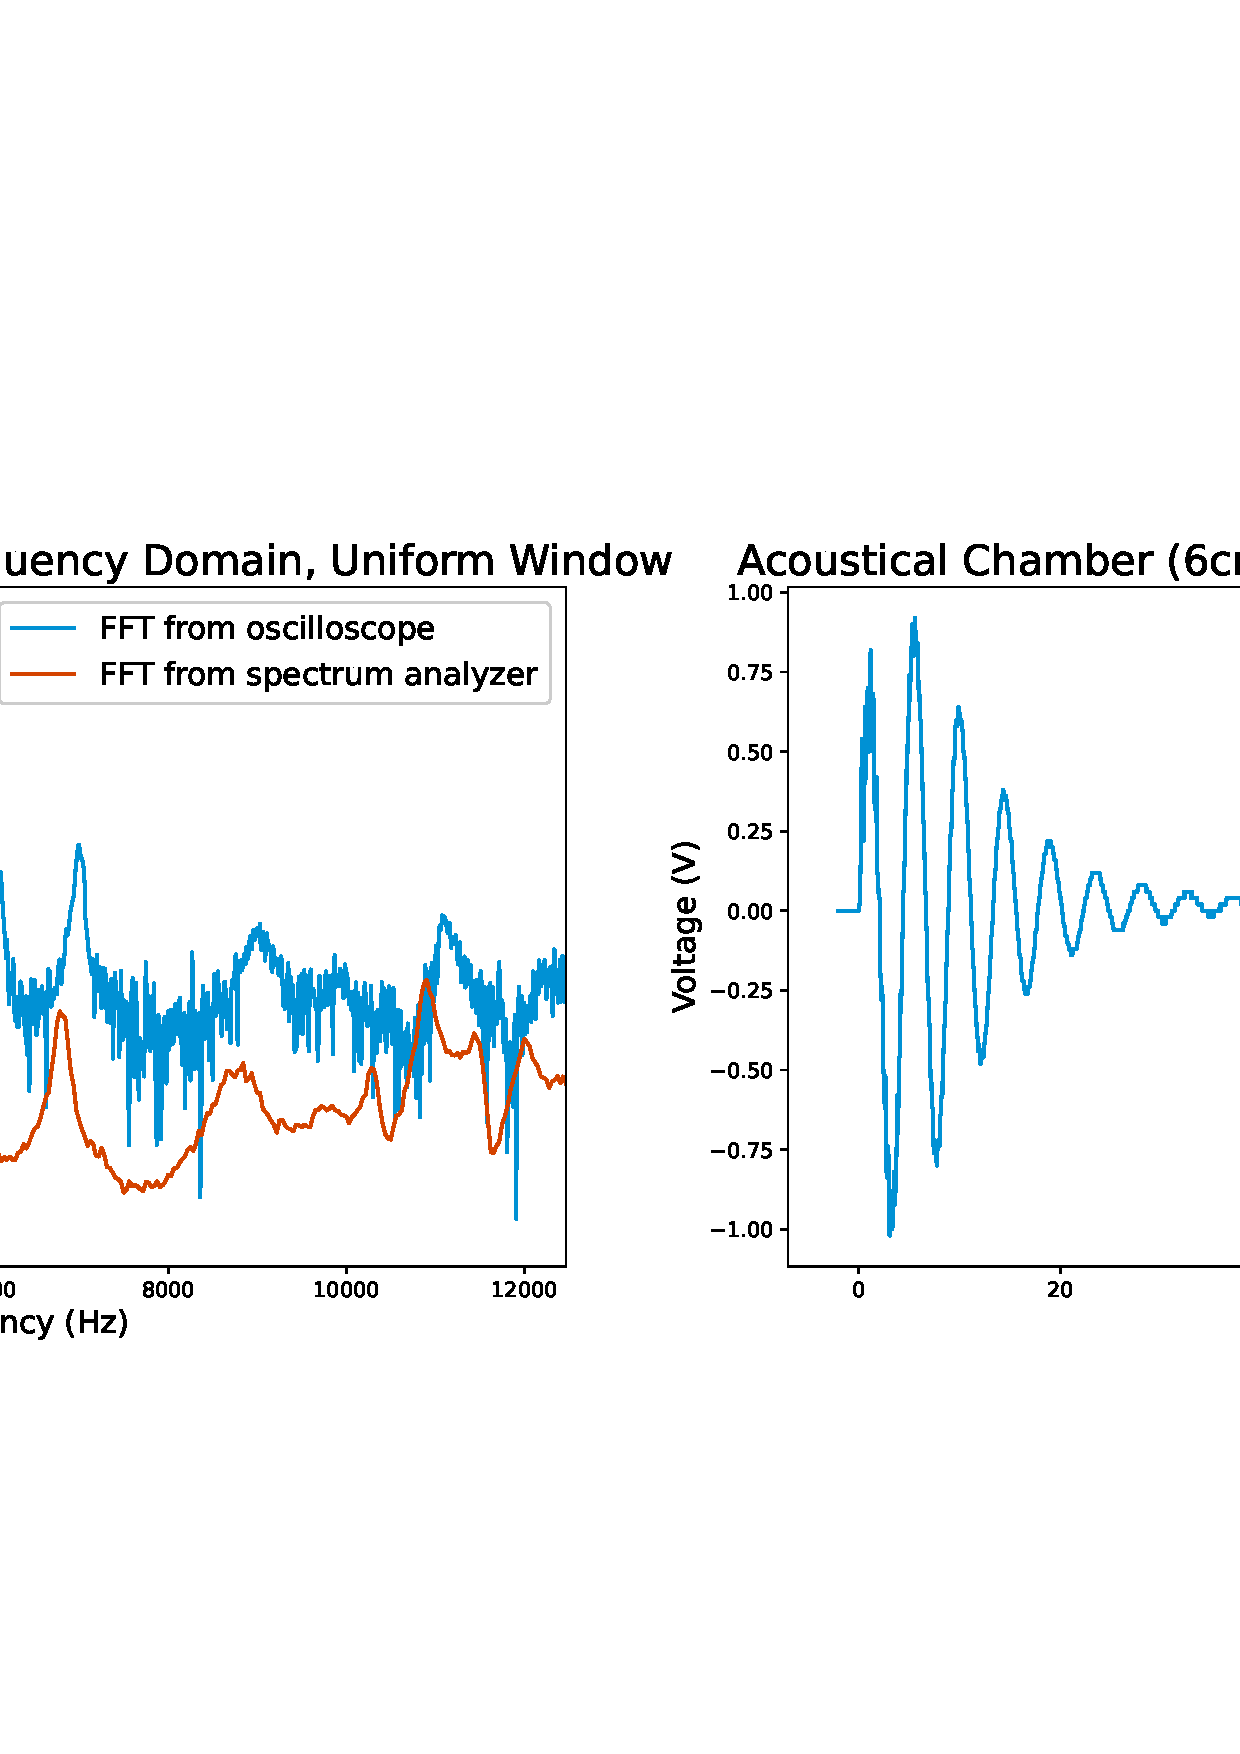
\includegraphics[width=\textwidth]{Acoustical Chamber (6cm) (uniform)}
    \caption{FFT analysis of the acoustical chamber. The data has not been trimmed, this may result in some noise. This serve also gives the possibility of an analysis of how a deadzone will effect the FFT. Here, it seems that there was not a considerable effect.}
    \label{fig:AC_fft}
\end{figure} % AC FFT


  
\begin{figure}[!ht]
    \centering
    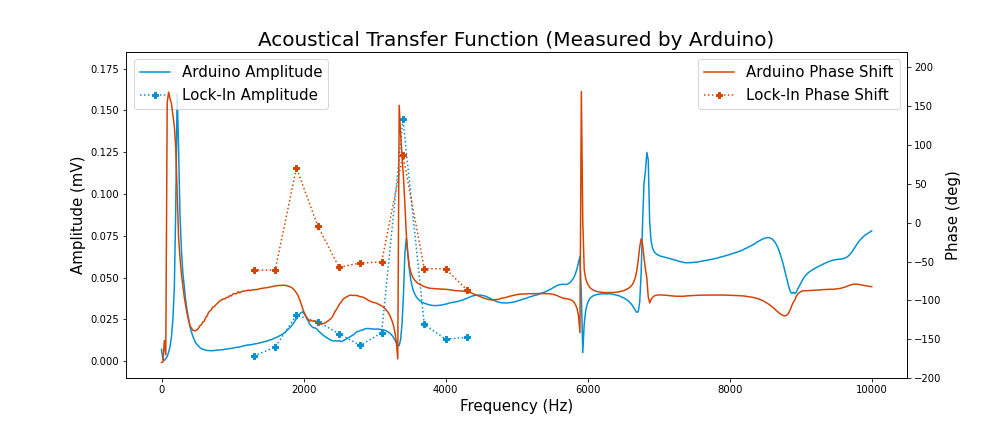
\includegraphics[width=\textwidth]{arduino data_0}
    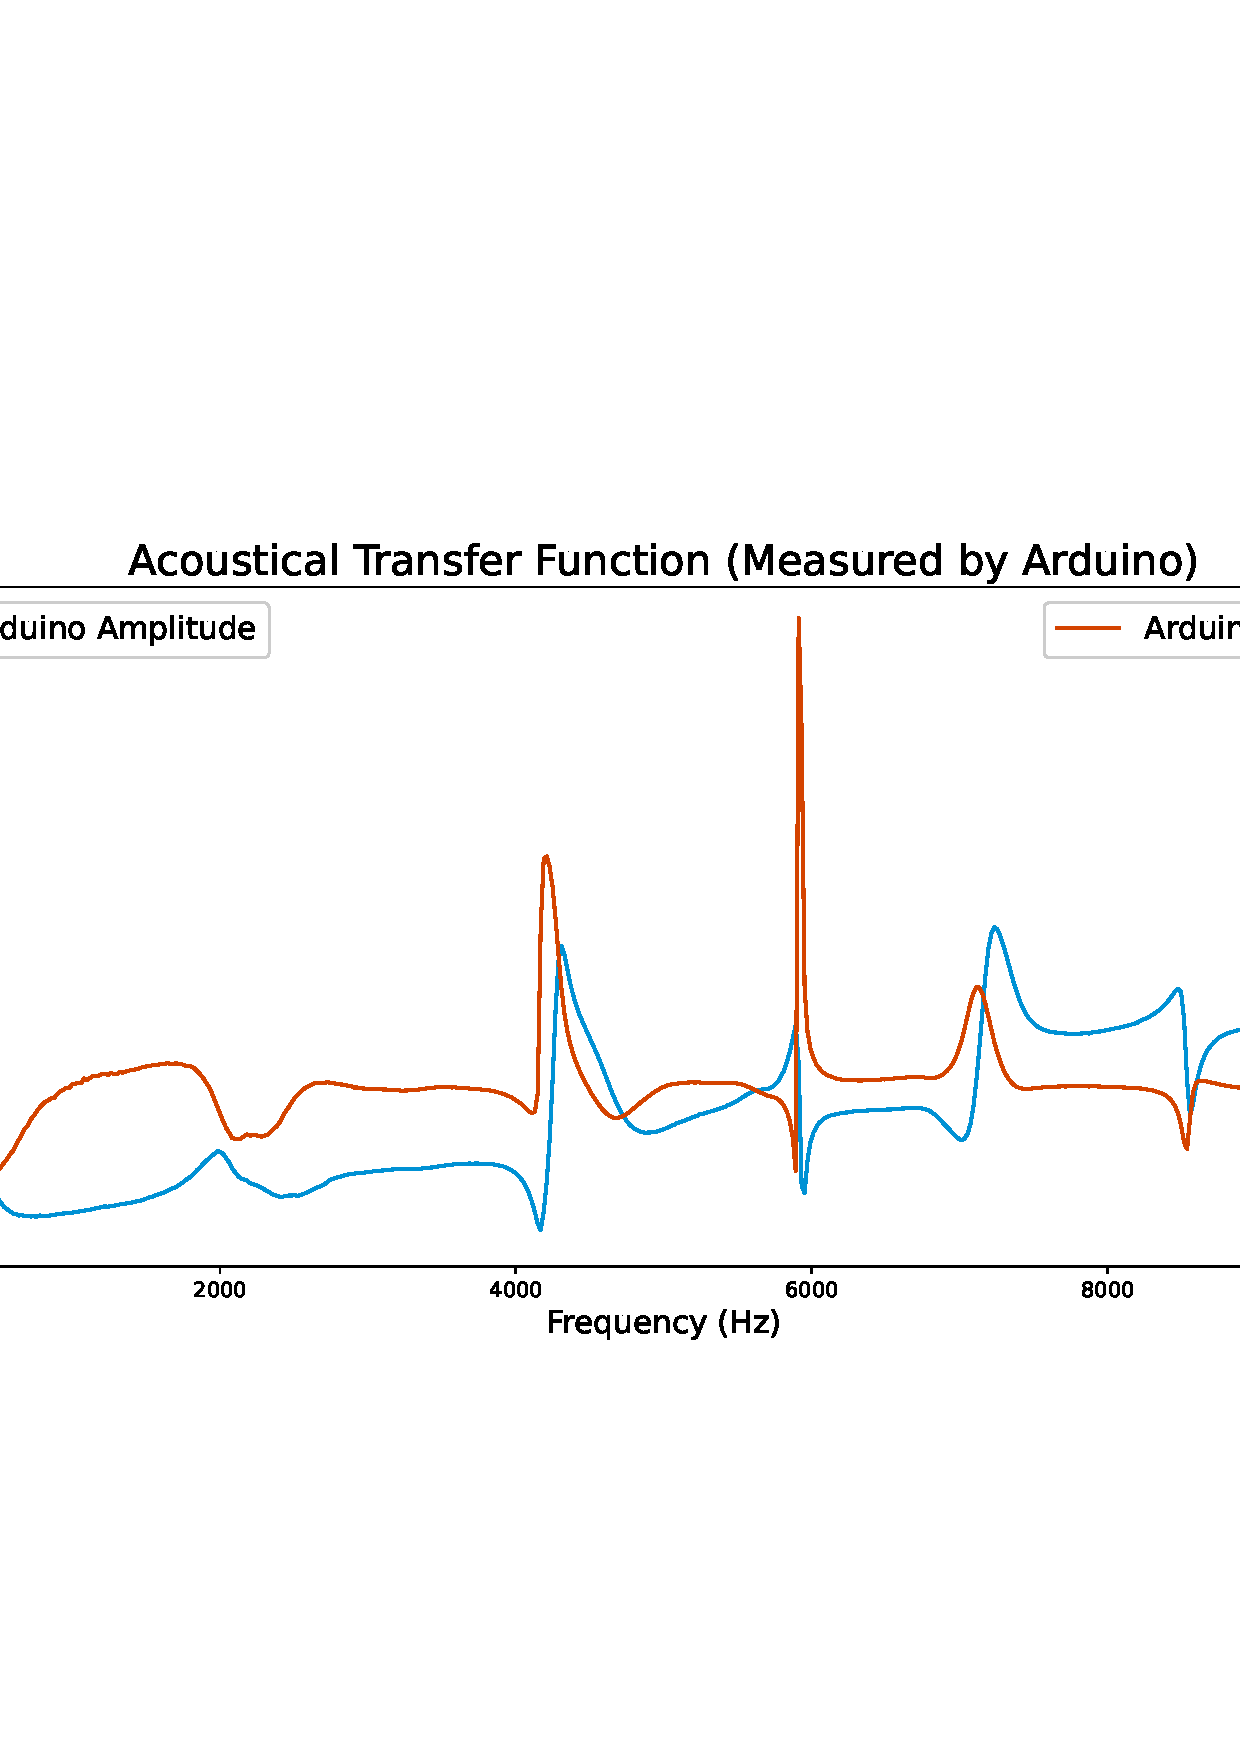
\includegraphics[width=\textwidth]{arduino data_1}
    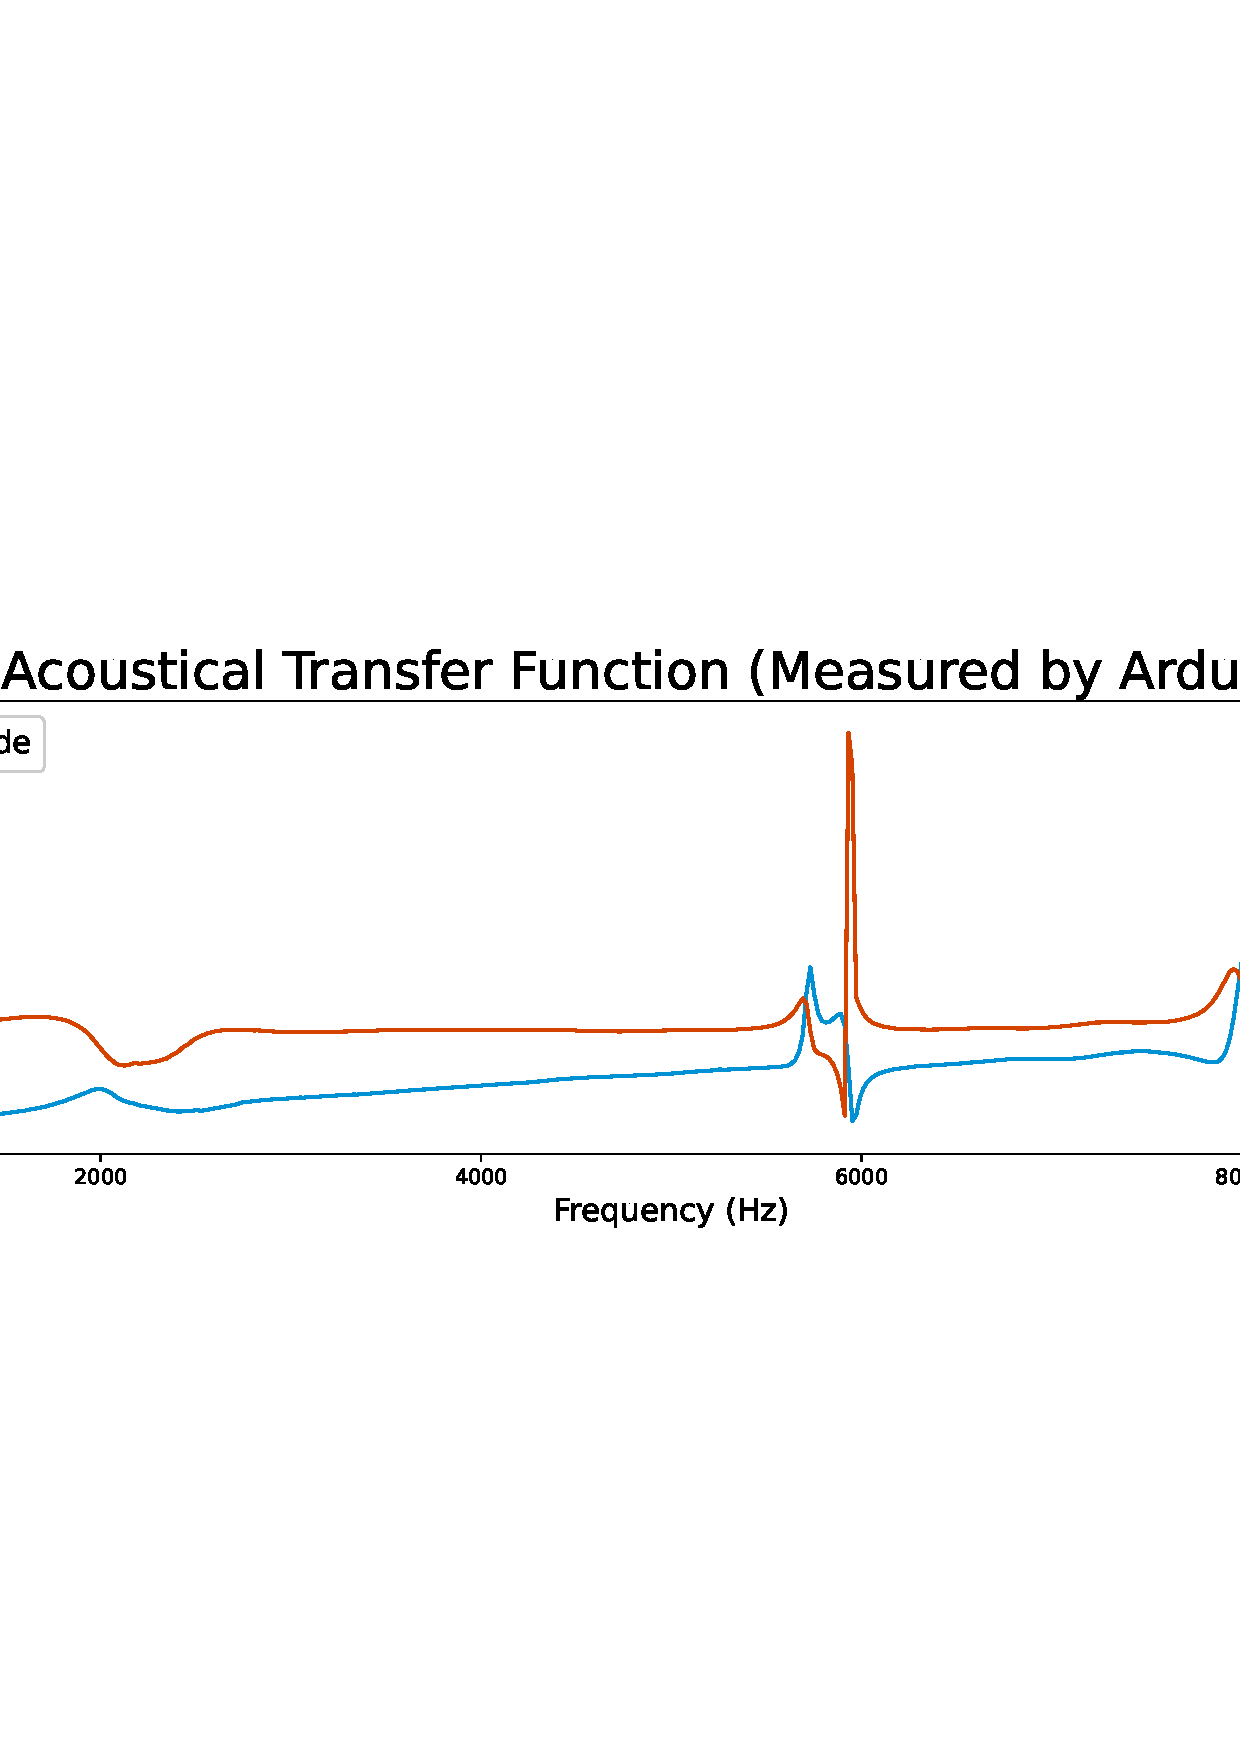
\includegraphics[width=\textwidth]{arduino data_2}
    \caption{Amplitude and Phase analysis from the Arduino and Lock-In Amplifier. it is interesting to note how similarly the amplitude and phase shift seem to travel together.}
    \label{fig:AC_Arduino}
\end{figure} % AC Arduino


\subsection{Acoustical Cavity Analysis}

The acoustical cavity seemed to provide a good example of a system with many different peaks, which were less predicatively spaced out. For each, the plot was loaded into a plotting software and the peaks were eyeballed according to a cursor's location. The values observed can be seen in Tables~\ref{tab:six_ac},~\ref{tab:five_ac},~\ref{tab:four_ac}, and~\ref{tab:three_ac}. As can be seen in those tables, the resonances found at the peaks all correspond very well. It should be noted that there are quite a few empty cells with missing data. These are from peaks not existing in those locations from the appropriate FFT. This is most likely due to not taking a long enough capture time or the seen peak being from shop noise. 

Again, the lock-in amplifier data was excluded from this analysis because there were not enough points to get a reliable measurement. It should be noted, however, that the amplifier's data showed similar results to both the amplitude and phase response as seen in the 6cm acoustical chamber. 

\begin{table}[!ht]
\centering
\begin{subtable}{0.45\textwidth}
\centering
\captionof{table}{6cm Acoustical Cavity} \label{tab:six_ac} 
	\begin{tabular}{c|c|c}
	Spec(Hz)&Osci(Hz)&Ardu(Hz)\\
	\hline
	202       & 205      & 210      \\
	2000      & 1991     & 1980     \\
	3435      & 3440     & 3440     \\
	4505      &          & 1410     \\
	5895      & 5930     & 5880     \\
	6772      & 6785     & 6800     \\
	8805      & 8825     & 8550     \\
	10305     &          &          \\
	10900     & 10900    &          \\
	11435     &          &          \\
	12035     & 12100    &         
	\end{tabular}
	\bigskip
\end{subtable}
\begin{subtable}{0.45\textwidth}
\centering
\captionof{table}{5cm Acoustical Cavity} \label{tab:five_ac} 
	\begin{tabular}{c|c|c}
	Spec(Hz)&Osci(Hz)&Ardu(Hz)\\
	\hline
	225        & 230       & 240       \\
	1990       & 1980      & 1990      \\
	           & 3280      &           \\
	4260       & 4260      & 4300      \\
	5905       & 5925      & 5890      \\
	7145       & 7200      & 7230      \\
	7205       &           &           \\
	8520       & 8530      & 8470      \\
	10500      & 9450      &           \\
	11050      & 11000     &           
	\end{tabular}
	\bigskip
\end{subtable}

\begin{subtable}{0.45\textwidth}
\centering
\captionof{table}{4cm Acoustical Cavity} \label{tab:four_ac} 
	\begin{tabular}{c|c|c}
	Spec(Hz)&Osci(Hz)&Ardu(Hz)\\
	\hline
	202    & 205     & 210    \\
	2000   & 1991    & 1980   \\
	3435   & 3440    & 3440   \\
	4505   &           & 1410   \\
	5895   & 5930    & 5880   \\
	6772   & 6785    & 6800   \\
	8805   & 8825    & 8550   \\
	10305  &           &          \\
	10900  & 10900   &          \\
	11435  &           &          \\
	12035  & 12100   &         
	\end{tabular}
	\bigskip
\end{subtable}
\begin{subtable}{0.45\textwidth}
\centering
\captionof{table}{3cm Acoustical Cavity} \label{tab:three_ac} 
	\begin{tabular}[t]{c|c}
	Spec(Hz)&Osci(Hz)\\
	\hline
	340         & 330        \\
	1950        & 1930       \\
	4550        & 4550       \\
	5930        & 5940       \\
	7100        &            \\
	8430        & 8480       \\
	10600       & 10600      \\             
	\end{tabular}
	\bigskip
\end{subtable}
\end{table}



  
\section{Discussion and Conclusions}
	Fourier Transforms are the basis to a lot of the data analysis used with modern experiments because of the unique insight into oscillatory information they provide. It is evident that post analysis can return compariable information to data taken live. This is a useful fact considering most systems can't be hooked up to a spectrum analyzer to be measured over a long time period. One such example being optically tracked particles in laser traps. 

	A couple points have been shown in this lab. The first being to be mindful of your $\Delta t$ and $t_{\text{max}}$. That point was the source of a lot of the errors, a prime example being the results of the Buried Treasure Module. Second, almost always consider applying a window function to the data before taking the FFT. In Figure~\ref{fig:LRC_fft} a window function was not used on the spectrum analyzer, and so one wasn't used on the oscilloscope FFT, consequently the data has an odd shape on it that doesn't provide much information past the primary peak. Finally, keep in mind the full picture of the test going on, and consider averaging over many tests. In the Acoustical Cavity Analysis, in Tables~\ref{tab:six_ac},~\ref{tab:five_ac},~\ref{tab:four_ac}, and~\ref{tab:three_ac} the various methods of data collection all gave slightly different sets of resonance frequencies. Averaging and considering background noise will help eliminate potential sources of extra peaks. If there is a known considerable source of noise, such as a running refrigerator upstairs, consider taking ``dark" data that only holds the noise data and systematically remove that from data taken in the future. 
	
	All together, this lab showed the power of using Fourier Transforms to get general transfer functions and points to keep in mind while applying them; not at all a trivial point.
   
   
   
   
\bibliographystyle{unsrt}
\bibliography{references}
   
\begin{thebibliography}{1}
    
    
\bibitem{circuit} “Circuit Diagram” Circuit Diagram, 2021. https://www.circuit-diagram.org/editor/. Accessed 21 Oct. 2021.
    
\bibitem{youtube} “The Fast Fourier Transform (FFT): Most Ingenious Algorithm Ever?” Reducible, YouTube, 14 Nov. 2020, https://www.youtube.com/watch?v=h7apO7q16V0. Accessed 30 Sept. 2021

\bibitem{hyper} Nave, R. Resonant RLC Circuits. Hyper Physics, 2019, hyperphysics.phy-astr.gsu.edu/hbase/electric/serres.html. Accessed 20 Oct. 2021.
‌
    
    
\end{thebibliography}
 
 
\newpage
\section*{Appendix A}
        
\begin{table}[!ht]
\centering
    \begin{tabular}{r|lll}
    Freq(Hz) & $X$(V)      & $Y$(V)      & Amp(V) \\
    \hline
    4.1  & 183.69 & 29.24  & 560 \\
    4.3  & 197.54 & 37.87  & 600 \\
    4.5  & 213.8  & 49.68  & 650 \\
    4.7  & 232.8  & 66.59  & 720 \\
    4.9  & 254.3  & 90.76  & 790 \\
    5.1  & 277.2  & 126.8  & 880 \\
    5.3  & 297.2  & 180.24 & 1010\\
    5.5  & 303.3  & 257.2  & 1140\\
    5.5  & 303.7  & 256.4  & 1140\\
    \end{tabular}
    \caption{Lock-In Amplifier data ($X$ and $Y$) and Oscilloscope (Amp) data collected for the appropriate frequency}
    \label{tab:lock_in_LRC}
\end{table}
    
    
\end{document}
